% !TeX spellcheck = en_US
% When submitting your files, remember to upload this *tex file, the pdf generated with it, the *bib file (if bibliography is not within the *tex) and all the figures.
%%%%%%%%%%%%%%%%%%%%%%%%%%%%%%%%%%%%%%%%%%%%%%%%%%%%%%%%%%%%%%%%%%%%%%%%%%%%%%%%%%%%%%%%%%%%%%%%%%%%%%%%%%%%%%%%%%%%%%%%%%%%%%%%%%%%%%%%%%%%%%%%%%%%%%%%%%%

%%% Version 3.4 Generated 2018/06/15 %%%
%%% You will need to have the following packages installed: datetime, fmtcount, etoolbox, fcprefix, which are normally inlcuded in WinEdt. %%%
%%% In http://www.ctan.org/ you can find the packages and how to install them, if necessary. %%%
%%%  NB logo1.jpg is required in the path in order to correctly compile front page header %%%

%\documentclass[utf8]{frontiersSCNS} % for Science, Engineering and Humanities and Social Sciences articles
%\documentclass[utf8]{frontiersHLTH} % for Health articles

\documentclass[utf8,sort&compress,table,hidelinks]{frontiersFPHY} % for Physics and Applied Mathematics and Statistics articles

\setcitestyle{square} % for Physics and Applied Mathematics and Statistics articles
\usepackage{url,hyperref,lineno,microtype,subcaption}
\usepackage[labelfont={bf,sf},%
labelsep=period,%
justification=centering,
labelformat=parens,labelsep=quad,skip=3pt,font=scriptsize]{caption}
\usepackage{graphicx}
\usepackage[onehalfspacing]{setspace}
\usepackage{multicol}
\usepackage[encoding,filenameencoding=utf8]{grffile}
\usepackage{xspace}
\usepackage{multirow}
\usepackage{booktabs}

\linenumbers

\newcommand{\thesi}{SI\xspace}
\newcommand{\tbd}{\textcolor{red}{TBD}\xspace}
\newcommand{\review}[1]{\textcolor{red}{#1}}

% Leave a blank line between paragraphs instead of using \\


\def\keyFont{\fontsize{8}{11}\helveticabold }
\def\firstAuthorLast{Coupette {et~al.}} %use et al only if is more than 1 author
\def\Authors{Corinna Coupette\,$^{1,\dagger}$, Janis Beckedorf\,$^{2,\dagger}$, Dirk Hartung\,$^{3,4,*}$,\\ Michael Bommarito\,$^{5}$, and Daniel Martin Katz\,$^{3,4,5}$}
% Affiliations should be keyed to the author's name with superscript numbers and be listed as follows: Laboratory, Institute, Department, Organization, City, State abbreviation (USA, Canada, Australia), and Country (without detailed address information such as city zip codes or street names).
% If one of the authors has a change of address, list the new address below the correspondence details using a superscript symbol and use the same symbol to indicate the author in the author list.
\def\Address{%
$^{\dagger}$These authors have contributed equally to this work and share first authorship.\\
$^{1}$Max Planck Institute for Informatics, Saarbr\"ucken, Germany\\ 
$^{2}$Ruprecht-Karls-Universit\"at Heidelberg, Heidelberg, Germany\\
\mbox{$^{3}$Center for Legal Technology and Data Science, Bucerius Law School, Hamburg, Germany}\\
$^{4}$CodeX -- The Stanford Center for Legal Informatics, Stanford Law School, CA,  USA\\
$^{5}$Illinois Tech -- Chicago Kent College of Law, Chicago, IL, USA
}
% The Corresponding Author should be marked with an asterisk
% Provide the exact contact address (this time including street name and city zip code) and email of the corresponding author
\def\corrAuthor{Dirk Hartung}

\def\corrEmail{dirk.hartung@law-school.de}


\graphicspath{ {./figures/} }

% UNCOMMENT FOR HANDIN
%\write18{cd figures && latexmk -pdf}

\begin{document}
\onecolumn
\firstpage{1}

\title[Measuring Law Over Time]{Measuring Law Over Time\newline\vspace*{-6pt}{\Large A network analytical framework with an application\newline to statutes and regulations in the United States and Germany}}

\author[\firstAuthorLast]{\Authors} %This field will be automatically populated
\address{} %This field will be automatically populated
\correspondance{} %This field will be automatically populated

\extraAuth{}% If there are more than 1 corresponding author, comment this line and uncomment the next one.
%\extraAuth{corresponding Author2 \\ Laboratory X2, Institute X2, Department X2, Organization X2, Street X2, City X2 , State XX2 (only USA, Canada and Australia), Zip Code2, X2 Country X2, email2@uni2.edu}


\maketitle


\begin{abstract}
\section{}
How do complex social systems evolve in the modern world? 
This question lies at the heart of social physics, 
and network analysis has proven critical in providing answers to it.
In recent years, network analysis has also been used to gain a quantitative understanding of law as a complex adaptive system, 
but most research has focused on legal documents of a single type, 
and there exists no unified framework for quantitative legal document analysis using network analytical tools.
Against this background, we present a comprehensive framework for analyzing legal documents as multi-dimensional, dynamic document networks. 
We demonstrate the utility of this framework by applying it to an original dataset of statutes and regulations from two different countries, the United States and Germany, spanning more than twenty years ($1998$--$2019$).
Our framework provides tools for assessing the size and connectivity of the legal system as viewed through the lens of specific document collections as well as for tracking the evolution of individual legal documents over time. 
Implementing the framework for our dataset, we find that at the federal level, the United States legal system is increasingly dominated by regulations, whereas the German legal system remains governed by statutes.
This holds regardless of whether we measure the systems at the macro, the meso, or the micro level. 


\tiny
 \keyFont{ \section{Keywords:} legal complexity, evolution of law, quantitative legal studies, empirical legal studies, legal data science, network analysis, natural language processing, complex systems} %All article types: you may provide up to 8 keywords; at least 5 are mandatory.
\end{abstract}

% !TeX spellcheck = en_US
% !TeX root = ../main.tex
\section{Introduction}
\label{sec:introduction}

Originating from mathematics and physics, complexity science has been successfully applied in the study of social phenomena \cite{mitchell2009,miller2009}. 
More recently, it was introduced as an approach to gain a quantitative understanding of the structure and evolution of law \cite{ruhl2017}. 
While legal scholars have long used concepts and terminology from complexity science in legal theory \cite{murray2018,ruhl1995,scott1993},
research has also called for the development of computational models, methods, and metrics to describe how law evolves in practice \cite{ruhl2015}.

Network analysis, a critical tool for understanding many complex systems \cite{amaral2004,albert2002,watts1998}, has proven particularly useful for scientific work answering this call.
It has been used, inter alia, to analyze network data derived from decisions by national courts \cite{coupette2019,winkels2019,black2013,lupu2013,bommarito2011,cross2010,fowler2007},
international courts \cite{olsen2020,alschner2018,larsson2017,tarissan2016a,panagis2015,pelc2014,lupu2012},
and international tribunals \cite{charlotin2017, langford2017},
as well as from statutes (i.e., rules promulgated by the legislative branch of government) \cite{katz2020,coupette2019a,boulet2018,koniaris2018,li2015,katz2014,bommarito2010},
constitutions \cite{lee2019,rutherford2018,rockmore2017},
and international treaties \cite{boulet2019,alschner2016,kim2013,kinne2013,saban2010}.
Relevant work in this context explored, for example, which characteristics of complex systems occur in statutory law \cite{katz2020,koniaris2018,li2015}, how references to judicial decisions are used to shape legal arguments \cite{larsson2017,black2013,lupu2013}, or where social dynamics exist between judges or international arbitrators \cite{katz2010,langford2017}.
The network analytical methods employed include centrality measures, clustering, and degree distributions \cite{katz2020,coupette2019,winkels2019,lee2019,alschner2016}.
However, while all studies examine network representations of legal document collections, the data models and methods employed vary widely, which makes it hard to assess the quality of individual results and compare findings across studies.
Furthermore, most of this research considers one legal document type only, 
and some important categories of legal documents, most prominently regulations (i.e., rules promulgated by the executive branch of government with authorization of the legislative branch of government), have---to the best of our knowledge---not received any network analytic attention.

This points to two gaps in the literature: 
First, on the methodological side, there exists no comprehensive framework for quantitative legal document analysis using network analytical tools.
Such a framework should be flexible in three ways:
It should (1) produce sensible results for different document types, countries, and time periods, 
(2) allow us to explore document collections of vastly different sizes, 
and (3) offer insights on the global (\emph{macro}), intermediate (\emph{meso}), and local (\emph{micro}) level of analysis. 
Second, on the empirical side, there is a lack of studies that combine multiple legal document types or include regulations.

In this article, we take a step toward filling both gaps.
We offer a comprehensive framework for analyzing legal documents as multi-dimensional, dynamic document networks 
and demonstrate its utility by applying it to an original dataset of statutes and regulations from two different countries, the United States and Germany, that spans more than twenty years ($1998$--$2019$).
Our framework provides tools for assessing the size and connectivity of the legal system as viewed through the lens of specific document collections as well as for profiling individual legal documents over time. 
It goes beyond the existing literature, inter alia, by adapting network analytical methods to the peculiarities of legal documents, allowing the joint examination of multiple document types, and enabling temporal analysis.
Implementing the framework for our dataset, we find that the United States legal system is increasingly dominated by regulations, 
whereas the German legal system remains governed by statutes, 
regardless of whether we measure the systems at the macro, the meso, or the micro level.

The remainder of the paper is structured as follows.
In Section~\ref{sec:data}, we specify our network model of legal documents and detail how we instantiate it to analyze statutes and regulations in the United States and Germany.
Section~\ref{sec:methods} describes our methodological framework,
and the results of applying this framework to our original dataset are presented in Section~\ref{sec:results}.
We conclude by discussing the strengths and weaknesses of our approach in Section~\ref{sec:discussion}, where we also identify avenues for future research. 
Our exposition uses the basic terminology of graphs and networks; for textbook introductions, see \cite{easley2010,barabasi2016,newman2018}.


% !TeX spellcheck = en_US
% !TeX root = ../main.tex
\section{Data}
\label{sec:data}

In this section, we introduce our network model of legal documents (\ref{subsec:data:model}) and instantiate it for our original dataset (\ref{subsec:data:instance}).

\vspace*{6pt}
\subsection{Data Model Specification}\label{subsec:data:model}

As visualized in Figure~\ref{fig:legal-system}~(a), the legal system consists of multiple levels: 
the local (e.g., municipal) level, the intermediate (e.g., state or province) level, the national (e.g., federal) level, and the supranational (including international) level.
Horizontally, it is usually subdivided into the legislative, executive, and judicial branches of government. 
These public parts are framed by the private sector, which operates on all levels, and the research community, which studies all parts of the legal system (including itself \cite{katz2011,newton2011,schwartz2011,george2006,ellickson2000}).
In all parts of the legal system, agents of varying sizes produce different types of outputs that create, modify, delete, apply, debate, or evaluate legal rules.
These agents and their typical outputs are summarized in Table~\ref{tab:legal-system}.

\begin{figure}
    \centering
    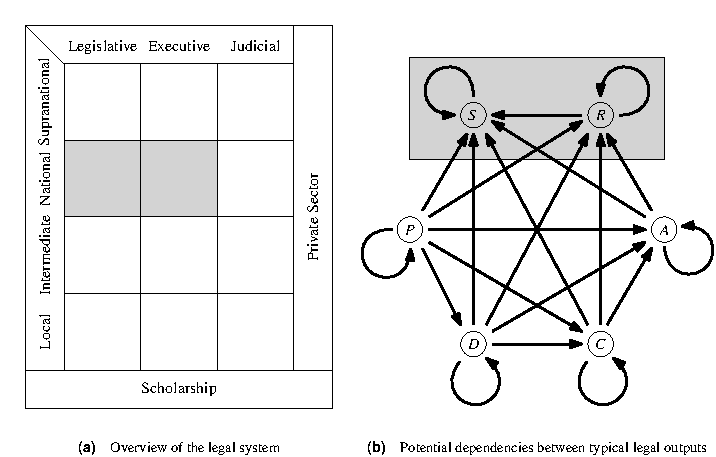
\includegraphics[width=\textwidth]{figure_1}
    \caption{Two-dimensional overview of the legal system (left) and dependencies between its typical outputs (right), with the areas covered by the dataset introduced in this work highlighted in grey. 
    The legal outputs in Panel~(b) are (clockwise from the top left and in reverse topological order) \textbf{S}tatutes, \textbf{R}egulations, Administrative \textbf{A}cts, \textbf{C}ontracts, (Court) \textbf{D}ecisions, and (Scholarly) \textbf{P}ublications.
    The arrows illustrate typical dependencies between the document types, e.g., through explicit references from arrow tails to arrow heads (although in reality, most dependencies can be bidirectional, e.g., some courts also cite legal scholarship). 
    Note that the sources covered by our dataset lie at the end of all typical dependency chains (i.e., statutes and regulations are last in the topological order of the dependency graph).
    }\label{fig:legal-system}
\end{figure}

 \begin{table}
	\centering
	\renewcommand{\arraystretch}{1.5}
\small
    \begin{tabular}{rllllll}
		\toprule&\multicolumn{3}{c}{\bfseries Branch of Government}&\bfseries Private Sector&&\bfseries Scholarship\\
		&\bfseries Legislative & \bfseries Executive & \bfseries Judicial&&&\\\midrule
		\bfseries Typical Large Agent&Parliament&Agency&Court&Firm&&Institute\\
		\bfseries Typical Small Agent&Parliamentarian&Bureaucrat&Judge&Individual&&Scholar\\
		\bfseries Typical Output(s)&Statute&Regulation&Decision&Contract&&Publication\\[-6pt]
		&&Administrative Act&&\\
		\bottomrule
	\end{tabular}

	\caption{Overview of agents and outputs in the legal system.}\label{tab:legal-system}
\end{table}

As the agents interact, they consciously interconnect their outputs. 
For example, court decisions regularly contain references to statutes, regulations, contracts, and other court decisions.
Figure~\ref{fig:legal-system}~(b) gives an overview of the classic dependencies between the typical outputs of agents in the legal system.
It illustrates that the \emph{documented} part of the legal system constitutes a multilayered document network, 
which is changing over time as the agents continue producing or amending their outputs.
Since the connections between the legal documents are placed deliberately by the agents, they encode valuable information about the content and the context of these documents. 
A lot of this information cannot be inferred from the documents' language alone (reliably or at all).
Therefore, investigating the dynamic document network representation of a legal system using network analytical tools promises insights into its structure and evolution that would be hard or impossible to obtain via other methods. 

To perform network analysis of a dynamic network of legal documents, we need to represent it as a series of graphs. 
Here, we build on a generalizable network model of statutory materials \cite{katz2020} and exploit the fact that the typical outputs listed in Table~\ref{tab:legal-system} have three common features (beyond the obvious characteristic that they all contain \emph{text}):
\begin{enumerate}
    \item They are hierarchically structured (\emph{hierarchy}).
    \item Their text is placed in containers that are sequentially ordered and can be sequentially labeled (\emph{sequence}).
    \item Their text may contain explicit citations or cross-references (henceforth: references) to the text in other legal documents or in other parts of the same document (\emph{reference}).
\end{enumerate}

Therefore, each document at a given point in time (henceforth: \emph{snapshot}) is represented as a (sub)graph, with its \emph{hierarchy} modeled as a tree using \emph{hierarchy edges}.
We capture a document's \emph{reference} using \emph{reference edges} at the level corresponding to the document's \emph{sequence}, which, inter alia, prevents the graph induced by these references from becoming too sparse (thereby eliminating some noise in the data and facilitating its analysis).
The result is a directed multigraph, as illustrated in Figure~\ref{fig:model} for documents that are statutes or regulations (whose sequence level is the \emph{section} level). 
Depending on the analytical focus, other edge types can be included (e.g., \emph{authority edges} pointing from regulations to statutes can indicate which statutes delegated the rule-making power used to create which regulations), 
and depending on the document types considered, different types of edit operations are possible (e.g., court decisions and scholarly articles are only seldom changed after their initial publication), 
but the general model applies to all outputs listed in Table~\ref{tab:legal-system}.

\begin{figure}
	\centering
	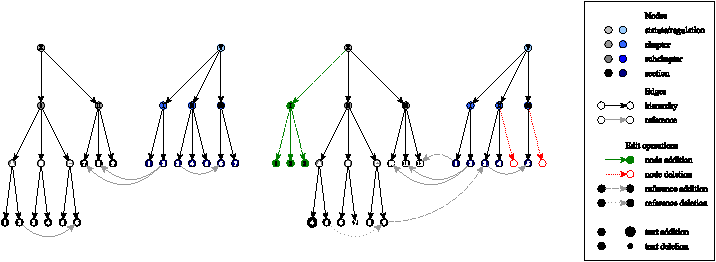
\includegraphics[width=\textwidth]{figure_2}
	\caption{Our legal network data model (adapted from \cite{katz2020}), illustrated for a dummy graph containing one statute and one regulation: initial configuration (left) and potential edit operations (right).}\label{fig:model}
\end{figure}

\vspace*{6pt}
\subsection{Data Model Instantiation}\label{subsec:data:instance}
To illustrate the power of the methodological framework laid out in Section~\ref{sec:methods} and produce the results presented in Section~\ref{sec:results}, we instantiate the data model described in Section~\ref{subsec:data:model} with the outputs of the legislative and executive branches of government at the national level in the United States and Germany, i.e., federal statutes and regulations, over the $22$~years from $1998$ to $2019$ (inclusive).
The rules contained in these sources are universally binding and directly enforceable through public authority (the combination of which distinguishes them from the other outputs listed in Table~\ref{tab:legal-system}).
In the United States and Germany, they are arranged into edited collections: the United States Code (USC) and the Code of Federal Regulations (CFR) in the United States, and the federal statutes and federal regulations (which have no special name) in Germany.
These collections are actively maintained to reflect the latest consolidated state of the law (though, in the United States, the consolidation may lag several years behind the actual law).
As such, they are a best-effort representation of all universally binding and directly enforceable rules at the federal level in their country at any point in time, commonly referred to as \emph{codified law}.

For the United States, we obtain the annual versions (reflecting the state of the codified law at the \emph{end} of the respective year) of the United States Code (USC) and the Code of Federal Regulations (CFR) from the United States Office of the Law Revision Council\footnote{\url{https://uscode.house.gov/download/annualhistoricalarchives/downloadxhtml.shtml}.} and the United States Government Publishing Office\footnote{\url{https://www.govinfo.gov/bulkdata/CFR}.}, respectively.
For Germany, we create a parallel set of annual snapshots for all federal statutes and regulations in effect at the \emph{end} of the year in question based on documents from Germany’s primary legal data provider, \emph{juris GmbH}.\footnote{
This differs from the approach taken in \cite{katz2020}, where the annual snapshots represented the law in effect at the \emph{beginning} of the year in question.
}
These data sources are the most complete presently available, 
but they may still be incomplete.
They also reflect choices made by and events affecting the agents in charge of their maintenance, e.g., varying rates and orders of updates, purposeful or unintentional omissions or modifications, and changes in the agents' composition (e.g., as a consequence of elections).

We perform several preprocessing steps on the raw input data, detailed in the Supplementary Information (\thesi), to extract the hierarchy, sequence, and reference structure contained in each collection.
The results are directed multigraphs, one per country and year, akin to those illustrated in Figure~\ref{fig:model}. 
These graphs contain all structural elements of the USC and the CFR (in the United States) or the federal statutes and regulations (in Germany) as nodes 
and all direct inclusion relationships (\emph{hierarchy}) and atomic references (\emph{reference}) as edges, where the references are resolved to the section level (\emph{sequence}).
Each graph represents the \emph{codified law} of a particular country in a particular year, containing documents of two \emph{document types} (statutes and regulations) at the federal level.

When modeling codified law as just described, we take a couple of design decisions that limit the scope of the results presented in Section~\ref{sec:results}. 
First, we focus on \emph{codified} law, i.e., \emph{law in books}, excluding other legal materials listed in Table~\ref{tab:legal-system}, especially those representing \emph{law in action} (in the sense of \cite{pound1910}),  
or even other representations of legislative materials such as the United States Statutes at Large or the German Federal Law Gazette (Bundesgesetzblatt).
These materials all merit investigation, and they need to be included in an all-encompassing assessment of the legal system. 
Our current work also serves as a preparatory step toward realizing this larger vision.

Second, we extract \emph{atomic} and \emph{explicit} references that follow a specified set of common patterns only, i.e., references including---in a typical format---a particular section (called ``Paragraph'' or ``Artikel'' in German law), a list of sections, or a range of sections.
With this procedure, we exclude \emph{container} references (e.g., references to an entire chapter of the USC), \emph{pinpoint} references (e.g., references to a codified Act of the United States Congress by its popular name), \emph{implicit} references (e.g., the use of a certain term implying its definition), and \emph{explicit} references following \emph{uncommon} patterns.
As sketched in Section~3.3 of the \thesi, there are plenty of such references, especially in the CFR, and including them would produce results different from those presented in Section~\ref{sec:results}.
However, the graph representation of such references is inherently ambiguous, 
and their extraction is inherently more challenging than the extraction of atomic citations.
Solving these problems falls outside the scope of this paper but presents an interesting opportunity for future work.

Third, we resolve the atomic references we extract to the level of sections, rather than the smallest referenced unit (which might be a subsection or even an item in an enumeration), thereby effectively discarding potentially valuable information.
Since for statutes and regulations, the section level corresponds to the documents' sequence level, this is consistent with our data model.
It also reflects a focus on the perspective of the user, who tends to navigate the law on the section level because it is the only level at which the individual German laws or their United States counterparts, the chapters of the USC and the CFR, are uniquely sequentially labeled. 
Finally, it ensures a certain degree of comparability because sections are the only structural elements in which text is (with very few exceptions) guaranteed to be contained (albeit the amount of text varies widely across sections).
Therefore, resolving references to the section level is reasonable for our purposes, but further research is needed on how the choice of the resolution level impacts the analysis of legal networks.


% !TeX spellcheck = en_US
% !TeX root = ../main.tex
\section{Methods}
\label{sec:methods}

Since the legal system produces a diverse set of outputs, many of which are rich in internal structure, a methodological framework for its dynamic network analysis must allow for many different foci and units of analysis. 
Our methods are designed to match this need, enabling us to describe the legal system and its evolution in its entirety (\emph{macro level}), through selected sets of legal documents (\emph{meso level}), or using individual documents and their substructures \emph{(micro level}), 
all while integrating documents of potentially different types.
More precisely, we provide tools for measuring 
\begin{enumerate}
	\item the \emph{growth} of the legal system (\ref{subsec:methods:growth}),
	\item the macro-level, meso-level, and micro-level \emph{connectivity} of the legal system (\ref{subsec:methods:connectivity}), and 
	\item the \emph{evolution} of individual units of law (e.g., single statutes, single regulations, or their sections or chapters) in the legal system (\ref{subsec:methods:profiles}).
\end{enumerate}
While most network analytical tools we employ are conceptually simple, the challenge lies in selecting adequate units of analysis and metrics allowing for substantive interpretation.
In the following, we refer to the object of study as \emph{the legal system} for brevity, 
but one should keep in mind that this system is explored through the window provided by the document collection underlying the analysis (cf.~Figure~\ref{fig:legal-system}), 
and therefore can also refer to a \emph{national legal system}.

\vspace*{6pt}
\subsection{Growth}
\label{subsec:methods:growth}

As detailed in Section~\ref{subsec:data:model}, despite their diversity, the typical outputs of the legal system have \emph{hierarchy}, \emph{sequence}, and \emph{reference} as common structural features, and they also all contain \emph{text}. 
Therefore, to assess the growth of the legal system, we track the number of tokens (roughly corresponding to words), the number of structural elements (i.e., hierarchical structures), and the number of references between documents of the same type at the documents' sequence level (e.g., the section level for statutes and regulations) across all documents in the collection, separately for each document type and across all temporal snapshots (e.g., all years). 
For the token counts, we concatenate the text of all materials for one snapshot and document type and split on whitespace characters. 
For a given document type, the structural element counts reflect the number of nodes of that type, and the reference counts reflect the number of reference edges between nodes of that type in our graphs.
These measures give a first, high-level idea of how the legal system evolves, and the aggregation by document type allows us to uncover, e.g., differences in growth rates. 

\begin{figure} 
	\centering
	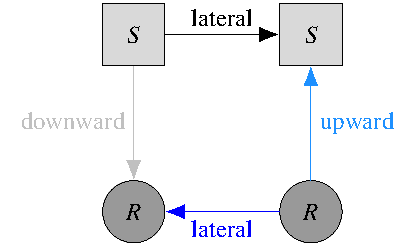
\includegraphics[width=0.5\textwidth]{figure_3}
	\caption{Differentiation of reference types for a document collection containing two types of documents: statutes and regulations. 
	Light grey squares marked $S$ represent sections of statutes, dark grey circles marked $R$ represent sections of regulations. 
	Given that statutes stand above regulations in the hierarchy of legal rules, 
	a reference from a statute to a regulation is \emph{downward} (silver), a reference from a regulation to a statute is \emph{upward} (light blue), 
	and references between documents of the same type are \emph{lateral} (black and blue).}\label{fig:crossref-differentiation}
\end{figure}

To explore the relevance of references between documents of different types, if the document collection contains $x$ types of documents, we distinguish between $x^2$ types of references. 
Figure~\ref{fig:crossref-differentiation} illustrates the idea for $x = 2$ with statutes and regulations as document types.
We count the number of references of each type for each temporal snapshot.

Raw reference counts do not show how the incoming and outgoing references are distributed across the individual sequence-level items. 
The user experience of a legal system, however, depends crucially on these distributions: 
If the typical item on the sequence level has very few outgoing references, the \emph{expected} cost of navigating the law is much smaller than if the outgoing references are uniformly distributed, 
and if the distribution of incoming references is very skewed, when reading the law, we are much more likely to encounter a few prominent sequence-level items than a large number of less prominent ones
(of course, the \emph{actual} cost of the user also depends on the size of the items to be navigated, which can vary widely, e.g., amongst the sections in the USC).
Therefore, we inspect the evolution of the in-degree distribution and the out-degree distribution of the subgraph induced by the reference edges.
We compute these distributions separately for each combination of reference edge types (e.g., considering any combination of the reference types depicted in Figure~\ref{fig:crossref-differentiation} for a document collection containing statutes and regulations) and across all snapshots.
This allows us to evaluate whether growth in the number of references further amplifies differences in the prominence of different parts of the law, 
which would be reflected in a lengthening or thickening of the distributions' tails, and to assess how this affects the navigability of a legal system.

\vspace*{6pt}
\subsection{Connectivity}
\label{subsec:methods:connectivity}

When exploring the connectivity of the legal system over time, we distinguish between macro-level connectivity (\ref{subsubsec:methods:connectivity:macro}), meso-level connectivity (\ref{subsubsec:methods:connectivity:meso}), and micro-level connectivity (\ref{subsubsec:methods:connectivity:micro}). 

\vspace*{6pt}
\subsubsection{Macro-level connectivity}
\label{subsubsec:methods:connectivity:macro}

Investigating connectivity at the macro level helps us understand how information in the legal system is organized and processed. 
As the basis of all analyses, we consider the graph induced by the structural items on the documents' sequence level (referred to as \emph{seqitems} in \cite{katz2020}) as nodes and the references between them as edges. 
For each snapshot, we count the number of non-trivial connected components (i.e., components with more than one node). 
Furthermore, we compute the fraction of nodes in the largest (weakly) connected component, 
the fraction of nodes in satellites, i.e., non-trivial components that are not the largest connected component, 
and the fraction of isolated nodes. 
We do this for the graph containing nodes of all document types as well as for the graphs containing only nodes of a single document type. 
These statistics provide a high-level overview of the system's information infrastructure and how it changes over time, 
and they enable a differentiated assessment of the role of documents of different types. 

For a more detailed picture, we draw on concepts introduced in the study of the Web graph \cite{broder2000}, which have also proven useful in the analysis of complex and self-organizing systems, e.g., in biology \cite{friedlander2015,csete2004,ma2003}. 
More precisely, we analyze the largest connected component of each of the sequence-level reference graphs, 
tracking the fraction of nodes contained in its strongly connected component, its in-only component (i.e., the nodes which can reach \emph{to} but cannot be reached \emph{from} the strongly connected component), its out-only component (i.e., the nodes which can be reached \emph{from} but cannot reach \emph{to} the strongly connected component), and its tendrils and tubes (whatever remains), 
again across all snapshots.
We ask to what extent the legal system has a bowtie structure (i.e., a small strongly connected core joined by larger in-only and out-only components), which has been associated with ``effective trade-offs among efficiency, robustness and evolvability'' \cite{csete2004}, inter alia, in complex biological systems, and whether any empirical deviations from that structure are characteristic of legal information processing.

\vspace*{12pt}
\subsubsection{Meso-level connectivity}
\label{subsubsec:methods:connectivity:meso}

One fundamental question concerning a legal system's connectivity at the meso level is how it self-organizes into areas of law.
Existing taxonomies categorizing the law into distinct fields are largely based on tradition (e.g., the titles of the USC) or intuition (e.g., the thematic categories used by some legal database providers). 
Exploiting the connectivity provided by references between legal documents at the meso level, network analytical methods provide an alternative, data-driven approach to mapping the law.
To implement such an approach, 
we follow a multi-step procedure:
\begin{enumerate}
	\item We preprocess the graphs for each snapshot by taking the quotient graph at the granularity we are interested in (e.g., at the level of individual chapters for an analysis of the USC and the CFR).
	That is, we remove all nodes above and below that level and reroute all references outgoing from or incoming to a lower-level node to the node's unique ancestor that lies on the level of interest.\label{step:quotient} 
	\item We cluster each of the \emph{undirected} versions of the graphs from Step~\ref{step:quotient} separately using the \emph{Infomap} algorithm \cite{rosvall2008,rosvall2009} with a parametrization that mirrors domain knowledge, and passes sensitivity and robustness checks. 
	Leveraging the randomness inherent in this algorithm, we increase the robustness of the clustering for each graph by computing the \emph{consensus clustering} \cite{lancichinetti2012} of $1000$ \emph{Infomap} runs with different seeds, where two nodes are put into the same cluster if they are in the same cluster in $95~\%$ of all runs.
	We choose the \emph{Infomap} algorithm as our clustering algorithm because it is scalable, has a solid information-theoretic foundation, and mirrors the process in which users like lawyers navigate law (inter alia, by identifying a relevant section of a statute, reading that section, then potentially following a reference).\label{step:clustering} 
	\item We compute pairwise alignments between the clusterings of all temporally adjacent snapshots based on the nodes of the \emph{unpreprocessed} graphs that wrap text (for details on our alignment procedure, see Section~4.3.1 in the \thesi).
	This is most relevant for collections containing documents that can change over time (e.g., statutes and regulations), and it allows us to assess, inter alia, what amount of text from a cluster $A$ in year $y$ is contained in a cluster $B$ in year $y+1$.\label{step:alignment}   
	\item We use the clusterings from Step~\ref{step:clustering} and the alignments from Step~\ref{step:alignment} to define a \emph{cluster family graph} as introduced in \cite{katz2020}. 
	This graph contains all clusters from all snapshots as nodes, and two clusters $A$ and $B$ are connected by a (weighted) edge if $A$ lies in snapshot $y$, $B$ lies in snapshot $y+1$, at least $p~\%$ of the tokens from $A$ are contained in $B$, and at least $p~\%$ of the tokens from $B$ are contained in $A$, where $p$ is chosen based on the analytical resolution we are interested in.\label{step:familygraph}
	\item We define a \emph{cluster family} as a connected component in a cluster family graph from Step~\ref{step:familygraph} and compute, for each cluster family in each year, the number of tokens it contains from each document type.\label{step:family}
\end{enumerate}
This process is a variant of the family graph construction developed for statutes in \cite{katz2020}, 
with the modification that we now allow for input data containing documents of different types.
It results in a dynamic, data-driven map of the legal system that accounts for the information provided by the references between its documents.

\vspace*{6pt}
\subsubsection{Micro-level connectivity}
\label{subsubsec:methods:connectivity:micro}

At the micro level, the connectivity created by references allows us to assess the roles of individual units of law. 
Regardless of the level at which we aggregate the references between documents, 
the shapes of the nodes' neighborhoods at that level contain valuable information about their function in the legal system. 
This information is partly accounted for in the meso-level connectivity assessment, which leverages local \emph{density}.
While local density can help us find out which nodes interact strongly, local \emph{sparsity} lets us identify nodes that play a particularly prominent role for the information flow in the network: 
If a node's neighbors are themselves only very sparsely connected (i.e., their neighbors almost form an independent set), the node provides an important \emph{bridge} between them.
We call the ego graph of such a node a \emph{star}, 
with the node as its \emph{hub} and the node's neighbors as the \emph{spokes}.

In directed graphs, we can classify stars according to the ratio between the hub's in-degree and the hub's out-degree as depicted in Figure~\ref{fig:star-types}.
More precisely, we define the type of a star $s$ with hub $v$ as follows:
\begin{align*}
	\text{type}(s) := \begin{cases}
		\frac{\delta^-(v)}{\delta^+(v)} \geq 10&\text{sink}\\
		\frac{1}{10} < \frac{\delta^-(v)}{\delta^+(v)} < 10&\text{hinge}\\
		\frac{\delta^+(v)}{\delta^-(v)} \geq 10&\text{source},
	\end{cases}
\end{align*}
where $\delta^+(v)$ is $v$'s out-degree and $\delta^-(v)$ is $v$'s in-degree.
In the legal system, the type of a star captures the hub's role in mediating the information flow in its neighborhood.

\begin{figure}
	\centering
	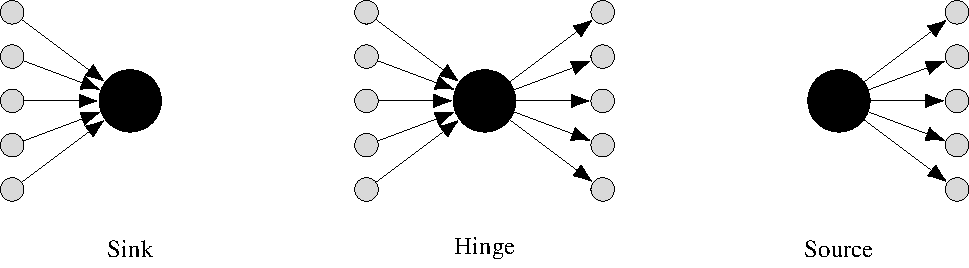
\includegraphics{figure_4}
	\caption{Star types. 
	If the hub's in-degree is at least ten times its out-degree, the star is a \emph{sink}. 
	If the hub's out-degree is at least ten times its in-degree, the star is a \emph{source}. 
	Otherwise, the star is a \emph{hinge}.}\label{fig:star-types}
\end{figure}

To identify and classify stars in the legal system at the documents' sequence level,
for each snapshot, we create the ego graph for each node $v$ in the graph induced by the reference edges (where we exclude parallel edges). 
We then iteratively remove the node $w$ that is connected to most of $v$'s neighbors while $w$ is connected to more than $5~\%$ of $v$'s neighborhood (excluding $w$), and keep the ego graph if it has a certain minimum size determined by the size of the collection (e.g., $10$ nodes for collections with several thousands of items on the sequence level).
The stars produced in this way contain no spoke that is connected to more than $5~\%$ of the other spokes, and we classify them to identify those sequence-level items that are vital to the information flow in their neighborhoods and to describe the type of mediation they perform.
To find stars at levels above the documents' sequence level, we can apply the methodology just described on graphs that aggregate references at those levels (e.g., on the quotient graphs described in Section~\ref{subsubsec:methods:connectivity:meso}).

\vspace*{12pt}
\subsection{Profiles}
\label{subsec:methods:profiles}

To assess the evolution of individual units of law (e.g., individual court decisions or chapters of a regulation) in the legal system, we create profiles of these units covering all temporal snapshots in the document collection under study.
More specifically, based on the quotient graphs that are created on the level of our unit of interest and contain only reference edges (like the preprocessed graphs described in Step~\ref{step:quotient}, Section~\ref{subsubsec:methods:connectivity:meso}), 
we track ten statistics in five groups (note that not all of these statistics can change over time for units of all legal document types):
\begin{enumerate}
	\item the number of tokens and the number of unique tokens,
	\item the number of items above, on, and below the sequence level (provided our unit of analysis lies above the sequence level),
	\item the number of self-loops,
	\item the weighted in- and out-degree (accounting for parallel edges), and
	\item the binary in- and out-degree (excluding parallel edges).
\end{enumerate} 

These statistics capture how the unit of law in focus evolves in size (number of tokens), 
topical breadth (number of unique tokens), 
structure (number of items above, on, and below the sequence level), 
self-referentiality (number of self-loops), 
scope of interdependence within the legal system (weighted in-degree and weighted out-degree), 
and diversity of interdependence within the legal system (binary in-degree and binary out-degree).
Finally, by constructing the ego graphs of the profiled unit for its out-neighborhood and its in-neighborhood and following the evolution of these ego graphs across snapshots,
we assess to what extent a profiled unit references which other units (\emph{reliance}) 
and to what extent it is referenced by which other units (\emph{responsibility}).


% !TeX spellcheck = en_US
% !TeX root = ../main.tex
\section{Results}
\label{sec:results}

In the following, we apply the framework presented in Section~\ref{sec:methods} to the data introduced in Section~\ref{subsec:data:instance}, i.e., codified law comprising federal statutes and regulations in the United States and Germany over the $22$ years from $1998$ to $2019$ (inclusive).
We start by examining the growth of the United States and German national legal systems (henceforth: the national legal systems) as viewed through the lens of our data (Section~\ref{subsec:results:growth}).
Next, we investigate the macro-level, meso-level, and micro-level connectivity of these national legal systems (Section~\ref{subsec:results:connectivity}).
Finally, we explore the evolution of selected chapters of the USC and the CFR and selected German statutes and regulations within their national legal systems in a case study focusing on financial regulation (Section~\ref{subsec:results:profiles}).
The results we report are mostly descriptive, and as discussed in Section~\ref{sec:discussion}, identifying causal factors behind the dynamics we observe or interpreting our results using a qualitative approach is left to future research.

\vspace*{30pt}
\subsection{Growth}
\label{subsec:results:growth}

Figure \ref{fig:basic-statistics} summarizes the growth of the United States legal system and the German legal system as measured by the tokens, structural elements, and lateral references contained in their codified law. 
Each row of the figure corresponds to a country, and each column corresponds to a document type. 
All counts are divided by their value in $1998$, i.e., Figure~\ref{fig:basic-statistics} depicts growth relative to the $1998$ baseline.
Supplementing the time series data, 
Table~\ref{tab:basic-statistics} provides the absolute counts for $1998$ and $2019$ and the total percentage change between these years ($\Delta$).

\begin{figure}
	\centering
	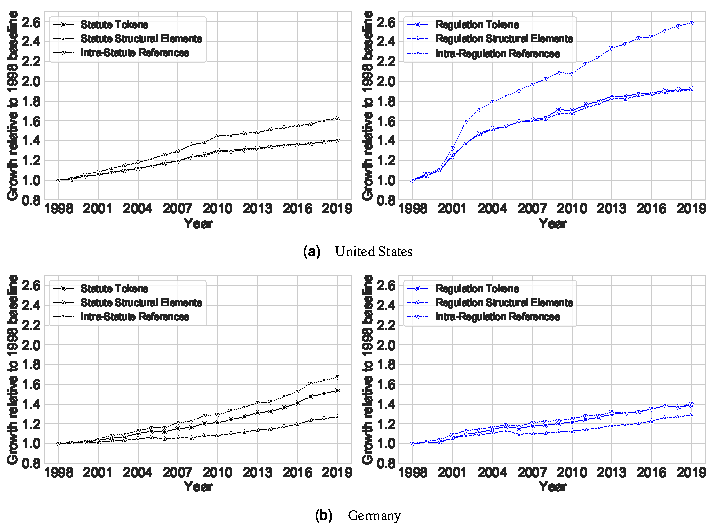
\includegraphics[width=\textwidth]{figure_5}
	\caption{Growth relative to the $1998$ baseline for statutes (left) and regulations (right) in the United States (top) and Germany (bottom).}\label{fig:basic-statistics}
\end{figure}

\begin{table}
	\centering
	% !TeX spellcheck = en_US
			\renewcommand{\arraystretch}{1.5}
				\begin{tabular}{lrrrrrr}
\toprule & \multicolumn{3}{c}{\textbf{Statutes}} & \multicolumn{3}{c}{\textbf{Regulations}} \\
            & 1998   & 2019   &   $\Delta$ & 1998   & 2019   &   $\Delta$ \\
\midrule
 \textbf{Tokens}     & 15.2~M               & 21.4~M               &                      41 & 43.9~M                  & 84.3~M                  &                         92 \\
 \textbf{Structures} & 516.2~K              & 838.8~K              &                      63 & 1.4~M                   & 2.7~M                   &                         91 \\
 \textbf{References} & 80.1~K               & 112.1~K              &                      40 & 134.6~K                 & 348.4~K                 &                        159 \\
\bottomrule
\end{tabular}
				
				{\vspace*{6pt}\small \textbf{\textsf{(a)}}\quad United States}\vspace*{12pt}
			
				\begin{tabular}{lrrrrrr}
\toprule & \multicolumn{3}{c}{\textbf{Statutes}} & \multicolumn{3}{c}{\textbf{Regulations}} \\
            & 1998   & 2019   &   $\Delta$ & 1998   & 2019   &   $\Delta$ \\
\midrule
 \textbf{Tokens}     & 5.0~M                & 7.7~M                &                      54 & 3.9~M                   & 5.4~M                   &                         39 \\
 \textbf{Structures} & 130.6~K              & 166.0~K              &                      27 & 87.9~K                  & 113.7~K                 &                         29 \\
 \textbf{References} & 86.4~K               & 144.6~K              &                      67 & 33.5~K                  & 47.1~K                  &                         41 \\
\bottomrule
\end{tabular}
				
				{\vspace*{6pt}\small \textbf{\textsf{(b)}}\quad Germany} 

	\caption{(Rounded) size of the national legal systems of the United States (top) and Germany (bottom) as measured by the tokens, structural elements, and references in their codified law in $1998$ and $2019$, including the total percentage change between these years ($\Delta$).}\label{tab:basic-statistics}
\end{table}

Figure~\ref{fig:basic-statistics} and Table~\ref{tab:basic-statistics} show that over the last two decades, the legal systems of both countries have grown substantially.  
In the United States, the USC (containing codified statutes) has over $60$ new structural elements (e.g., chapters, parts, or sections) in $2019$ for every $100$ such elements it had in $1998$.
Notably, as evident from the upper left panel of Figure~\ref{fig:basic-statistics}, the growth rate of the USC appears to have experienced two distinct periods when measured by its structural elements: 
one period with a monotonic growth rate of approximately $4~\%$ per year ($1998$--$2010$), followed by another period with a decelerated monotonic growth rate of approximately $2~\%$ per year ($2010$--$2019$). 
At a slightly lower level, this trend also occurs for both the number of tokens and the number of intra-USC references. 
For example, there are approximately $40$ new tokens or references in $2019$ for every $100$ tokens or references that existed in $1998$.
Shifting the focus for the United States to the CFR (containing codified regulations), as observable from the upper right panel of Figure~\ref{fig:basic-statistics}, the quantity of regulations has increased by an even greater factor.  
For every $100$ structural elements or tokens that were present in $1998$, approximately $90$ additional elements or tokens exist in $2019$. 
This increase is even more extreme for intra-CFR references, where there are almost $160$ \emph{new} references in $2019$ for every $100$ that existed in $1998$.  
Apart from brief intervals of stagnation or slight decrease ($2009$--$2010$, $2013$--$2014$), 
these increases have been monotonic.

Corresponding trends for German statutes and regulations are presented in the bottom row of Figure \ref{fig:basic-statistics}.  
Growth in the German legal system has been qualitatively similar to that in the United States legal system but quantitatively less pronounced and of different functional shape. 
For both German statutes and German regulations, there are approximately $30$ new structural elements in $2019$ for every $100$ that existed in $1998$. 
Unlike in the United States, however, this growth has been non-monotonic: 
When measured through structural elements, both statutes and regulations experienced some periods of shallow decline between $2005$ and $2010$.
These shrinking periods are generally not mirrored by the token and lateral reference counts, with one notable exception:
In the period from $2005$ to $2006$, \emph{all} German statistics decreased. 
This is likely due to statutes aiming to cleanse the law (\emph{Rechtsbereinigungsgesetze}), eight of which were introduced in $2006$ (recall that our $2006$ snapshot represents the law at the \emph{end} of $2006$).\footnote{%
These statutes are: 
(1) Erstes Gesetz über die Bereinigung von Bundesrecht im Zuständigkeitsbereich des Bundesministeriums des Innern vom 19. Februar 2006 (BGBl.~I~S.~334),
(2) Gesetz zur Bereinigung des Bundesrechts im Zuständigkeitsbereich des Bundesministeriums für Ernährung, Landwirtschaft und Verbraucherschutz vom 13. April 2006 (BGBl.~I~S.~855),
(3) Erstes Gesetz über die Bereinigung von Bundesrecht im Zuständigkeitsbereich des Bundesministeriums der Justiz vom 19. April 2006 (BGBl.~I~S.~866),
(4) Erstes Gesetz zur Bereinigung des Bundesrechts im Zuständigkeitsbereich des Bundesministeriums für Wirtschaft und Technologie und im Zuständigkeitsbereich des Bundesministeriums für Arbeit und Soziales vom 19. April 2006 (BGBl.~I~S.~894),
(5) Gesetz zur Änderung und Bereinigung des Lastenausgleichsrechts vom 21. Juni 2006 (BGBl.~I~S.~1323),
(6) Gesetz über die Bereinigung von Bundesrecht im Zuständigkeitsbereich des Bundesministeriums für Arbeit und Soziales und des Bundesministeriums für Gesundheit vom 14. August 2006 (BGBl.~I~S.~1869),
(7) Erstes Gesetz über die Bereinigung von Bundesrecht im Zuständigkeitsbereich des Bundesministeriums für Verkehr, Bau und Stadtentwicklung vom 19. September 2006 (BGBl.~I~S.~2146), and
(8) Zweites Gesetz über die Bereinigung von Bundesrecht im Zuständigkeitsbereich des Bundesministeriums des Innern vom 2. Dezember 2006 (BGBl.~I~S.~2674).
}
In total, there are approximately $55$ new statute tokens in Germany in $2019$ for every $100$ such tokens that existed in $1998$. 
Like \emph{regulations} in the United States, German \emph{statutes} experienced a greater increase in the quantity of lateral references than in other metrics: 
For every $100$ references in $1998$, there are approximately $70$ new references in $2019$. 
For German \emph{regulations}, as for \emph{statutes} in the United States, the rate of change has been more similar across metrics, with growth varying roughly between $30~\%$ and $40~\%$ (as noted in Table~\ref{tab:basic-statistics}).
At a high level, the growth of the German legal system thus seems to be driven by statutes, whereas the growth of the United States legal system appears to be driven by regulations.

\begin{figure}
	\centering
	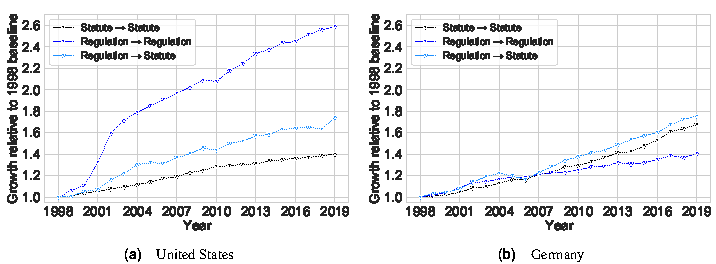
\includegraphics[width=\textwidth]{figure_6}
	\caption{Growth relative to the $1998$ baseline for lateral and upward references in the United States (left) and Germany (right).}\label{fig:crossref-evolution}
\end{figure}

Figure~\ref{fig:basic-statistics} and Table~\ref{tab:basic-statistics} only account for \emph{lateral} references, excluding references between documents of different types. 
Therefore, Figure~\ref{fig:crossref-evolution} shows growth relative to the $1998$ baseline for lateral and \emph{upward} (i.e., regulation-to-statute) references. 
We exclude \emph{downward} references because they are very few in number (which means that even a small absolute increase results in a large relative increase) 
but note that, contrary to the legal theory intuition, they \emph{do} occur.\footnote{%
The total number of downward references in the United States increases from $24$ in $1998$ to $90$ in $2019$.
In Germany, it rises from $305$ to $833$.
}
As evident from Figure~\ref{fig:crossref-evolution}, upward references have grown at similar rates in both countries, with approximately $80$ new upward references existing in $2019$ for every $100$ upward references that existed in $1998$. 
This relative increase is larger than that of the lateral references in both countries, with the exception of lateral regulation references in the United States, whose growth rate dwarfs all others. 
Since the token and structural element growth rates of German regulations are lower than or similar to those of German statutes, this means that over the period under study, connectivity between statutes and regulations in Germany has grown faster than connectivity within statutes or within regulations. 

To evaluate how the growth in the number of references affects the differences in the prominence of individual sections of codified law in the legal systems under study, in Figure~\ref{fig:degree-distribution}, we examine the in-degree distribution and the out-degree distribution of the graphs induced by the reference edges in $1998$ and $2019$ (an analogous figure normalizing section degrees by section size in tokens can be found in Section~4.1 of the \thesi).  
Since these distributions are highly skewed (as in many graphs arising from complex systems), we plot them on a log-log scale. 

\begin{figure}
	\centering
	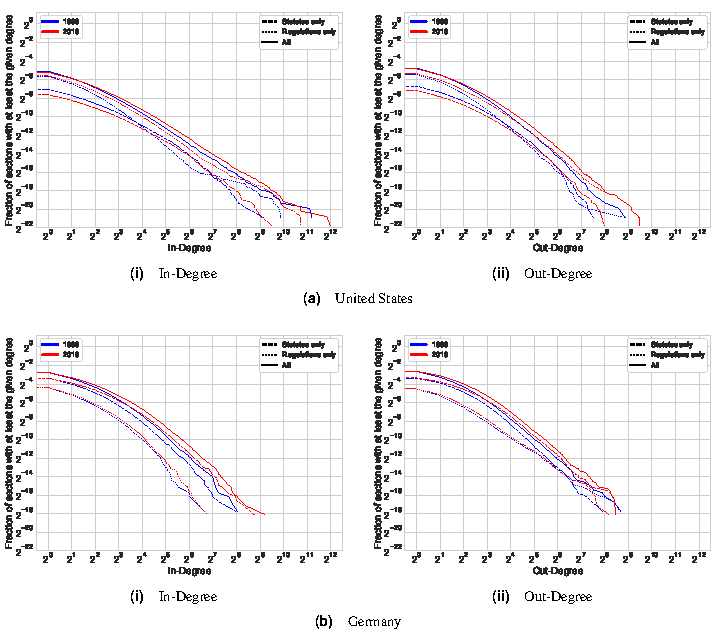
\includegraphics[width=\textwidth]{figure_7}
	\caption{In-degree (left) and out-degree (right) distributions for the United States (top) and Germany (bottom) in $1998$ (blue) and $2019$ (red) when considering statutes only (dashed line), regulations only (dotted line), or statutes and regulations (solid line).}\label{fig:degree-distribution}
\end{figure}

All distributions plotted in Figure~\ref{fig:degree-distribution} demonstrate features common among graphs arising from bibliometric dynamics. 
For example, most sections of statutes and regulations in the United States and Germany are referenced very few times (if at all). 
The detailed characteristics of the distributions, however, differ between distribution types, document types, and countries:
For the United States, the out-degree distributions exhibit less right skew than their in-degree counterparts, 
while in Germany, we observe the opposite: 
All out-degree distributions are either within an order of magnitude of or have a longer and thicker right tail than their in-degree counterparts. 
Similarly, the sections contained in United States regulations exhibit a higher degree of skew in their in-degree distributions than the sections contained in United States statutes 
(e.g., a higher fraction of these sections has more than $500$ ingoing references), 
but in Germany, the opposite phenomenon occurs at a lower absolute level: 
There are many statute sections with more than $100$ ingoing references but hardly any regulation sections clearing that threshold. 
These national divergences might be partly due to the differing ratio between statutes and regulations, but they could also point to peculiarities in United States and German drafting style.

Comparing \emph{all} distributions across countries, we observe that the United States legal system exhibits more extreme statistics than the German legal system (which might, at least in part, be due to its larger size).
Finally, we see that from $1998$ to $2019$, most distributions shift to the right, i.e., the tails become both longer and thicker, 
which is in line with bibliometric preferential attachment dynamics \cite{merton1968,price1976}.
This indicates that reference growth has disparate impact, amplifying the differences in relevance between the individual sections contained in United States and German statutes and regulations.
As a consequence, the difficulty of navigating the law increases more slowly than the growth of the reference count may suggest. 

\vspace*{12pt}
\subsection{Connectivity}
\label{subsec:results:connectivity}

When exploring the connectivity of the national legal systems of the United States and Germany over time, we distinguish between the macro level, the meso level, and the micro level as suggested in Section~\ref{subsec:methods:connectivity}.

\vspace*{6pt}
\subsubsection{Macro-level connectivity}
\label{subsubsec:results:connectivity:macro}

To understand how the United States legal system and its German counterpart organize and process information, we investigate the connectivity of the graphs containing code sections as nodes and references between them as edges. 
Figure~\ref{fig:connectivity-components} displays the number of non-trivial (weakly) connected components (i.e., components with more than one node) in these graphs over time, 
in absolute terms and per $1000$ tokens.
It shows that the connectivity in the graphs containing only statute sections is generally higher than that in the graphs containing only regulation sections or sections of both document types.
Furthermore, while the United States system seems more fragmented than the German system (Figure~\ref{fig:connectivity-components}~(a)) when considering absolute numbers, it turns out to be relatively less fragmented when normalizing for system size (Figure~\ref{fig:connectivity-components}~(b)).

\begin{figure}
	\centering
	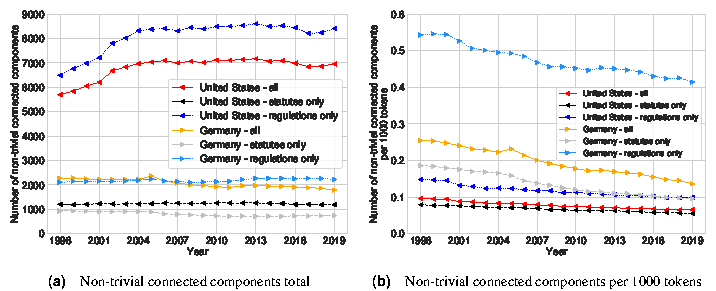
\includegraphics[width=\textwidth]{figure_8}
	\caption{Development of reference connectivity as measured by the absolute number of non-trivial (weakly) connected components (left) and the number of non-trivial (weakly) connected components per $1000$ tokens (right) in the graphs induced by reference edges between all sections (solid lines), statute sections only (dashed lines), and regulation sections only (dotted lines) in the United States (left-pointing triangles) and Germany (right-pointing triangles).}\label{fig:connectivity-components}
\end{figure}

For a more granular connectivity assessment over time, Figure~\ref{fig:connectivity-all} shows, for each year from $1998$ to $2019$, what fraction of statute sections and regulation sections in each country is contained in the largest connected component, satellite components, or isolates, 
and how the largest connected component is composed internally. 
The underlying graphs do not distinguish between sections of different document types; 
analogous figures considering statute sections only and regulation sections only can be found in Section~4.2 of the \thesi.
In both the United States and Germany, the largest connected component is growing as the fraction of sections contained in both satellites and singletons decreases, 
and the difference between the largest connected component fraction in $1998$ and that in $2019$ is around $10~\%$. 
However, the relative size of these largest connected components varies substantially between the two countries: 
In the United States, the largest connected component has grown from about $40~\%$ to nearly $50~\%$, 
while in Germany, its size has increased from circa $55~\%$ to roughly $65~\%$.
Furthermore, the fraction of isolates (sections that neither reference another section nor get referenced by another section) is larger in the United States (around $45~\%$ in $2019$) than in Germany (below $30~\%$ in $2019$).

\begin{figure}
	\centering
	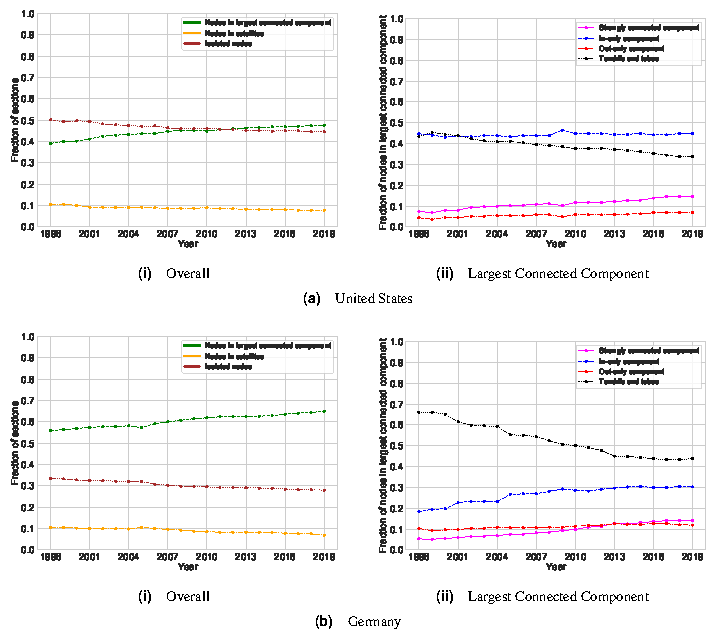
\includegraphics[width=\textwidth]{figure_9}
	\caption{Development of reference connectivity in the United States (top) and Germany (bottom) as measured by the fraction of sections contained in the largest connected component (left), along with the internal structure of that component (right).}\label{fig:connectivity-all}
\end{figure}

When focusing on the largest connected component and taking edge directions into account, the differences between the two countries become even more pronounced.  
In the United States, the fraction of the largest connected component contained in the in-only component is almost equal to that contained in its tendrils and tubes in $1998$, and both lie around $45~\%$.
Over time, these fractions diverge as the strongly connected component and the out-only component grow and the in-only component stagnates. 
In Germany, however, tendrils and tubes dominate in $1998$, accounting for more than $65~\%$ of nodes, 
but by $2019$, their fraction has declined to less than $45~\%$, while the strongly connected component and the out-only component have grown at low levels and the in-only component has gained more than $50~\%$ in fractional size (growing from less than $20~\%$ to over $30~\%$).

Notably, in both legal systems, the out-only component accounts for the smallest fraction of sections in $2019$ (around $7~\%$ in the United States and around $12~\%$ in Germany), followed by the strongly connected component, with none of them containing more than $15~\%$ of all sections, while the in-component is twice as large in Germany and thrice as large in the United States.
Hence, at least when considering code sections as nodes and references between them as edges, both national legal systems do not exhibit the bowtie structure observed in biological systems (small strongly connected component with larger in-only and out-only components \cite{friedlander2015}) or that found in early measurements of the World Wide Web (all components, including tendrils and tubes, of roughly the same size, with a slightly larger strongly connected component \cite{broder2000}).
Rather, the legal systems we study are shaped more like rockets, with the in-only component as their base, tendrils and tubes as their fins, the strongly connected component as their body, and the out-component as their nose cone (see Figure~\ref{fig:rocket} for an illustration).
The rocket structure mirrors both the hierarchical structure of legal systems (large in-only component, small out-only component) and the fact that some areas of law function relatively independently (many tendrils and tubes; also evident from the nontrivial fraction of nodes outside the largest connected component). 
This suggests that it might be characteristic of legal systems in general, but more research is needed to corroborate this hypothesis.
Similarly, it would be interesting to investigate how our observations change if we include, e.g., non-atomic references (which, by definition, interconnect multiple sections).

\begin{figure}[h]
	\centering
	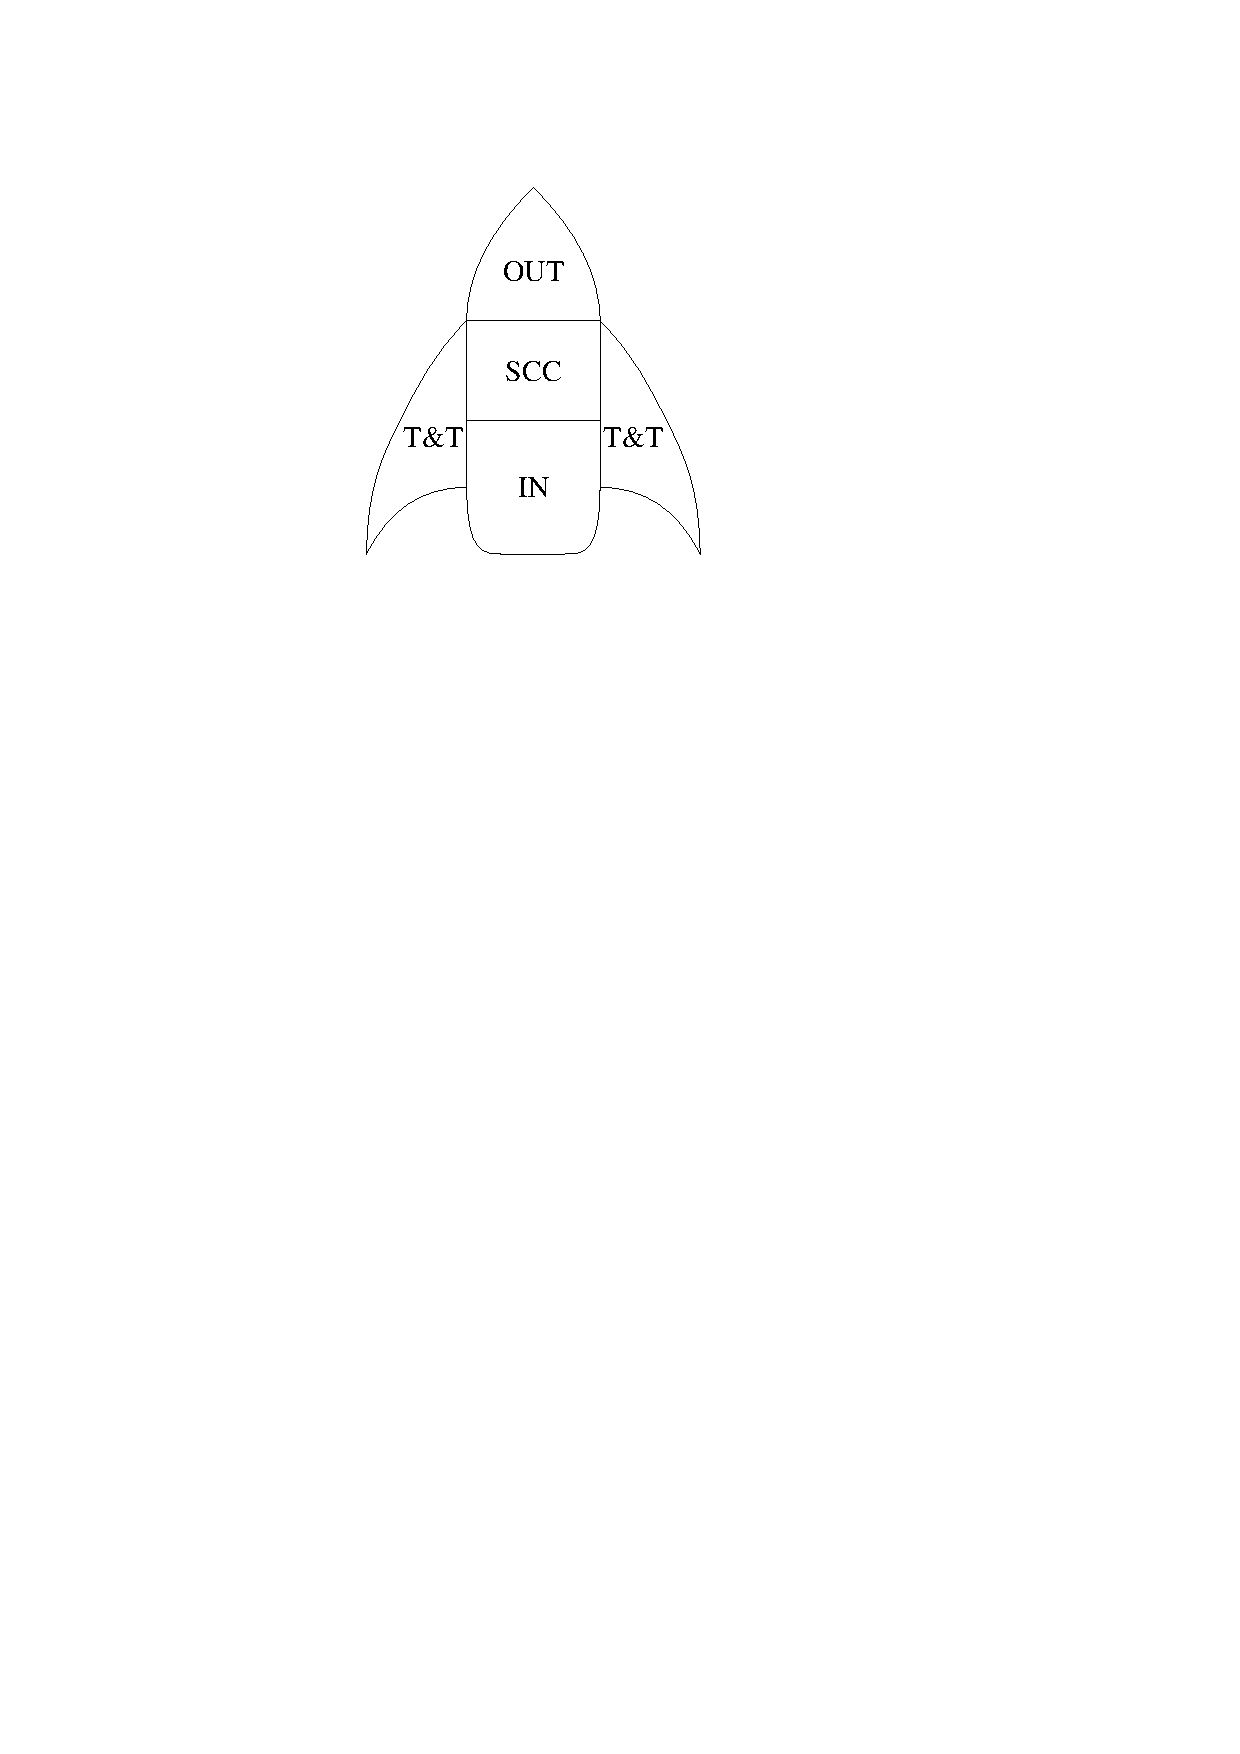
\includegraphics{figure_10}
	\caption{Rocket structure of a legal system when viewed through the lens of macro-level connectivity, with the in-component (IN) as the rocket's base, the strongly connected component (SCC) as the body, the out-component (OUT) as the nose cone, and tendrils and tubes (T\&T) as the fins.}\label{fig:rocket}
\end{figure}

\vspace*{12pt}
\subsubsection{Meso-level connectivity}
\label{subsubsec:results:connectivity:meso}

When analyzing the connectivity of the United States and German legal systems at the meso level, our goal is to create a dynamic, data-driven map of their codified law.
To this end, for both the United States and Germany, we compute cluster families as described in Section~\ref{subsubsec:methods:connectivity:meso}, 
using quotient graphs on the chapter level in the United States and on the statute or regulation level (or the book level, if available) in Germany. 
Here, we choose $100$ as the preferred number of \emph{Infomap} clusters and $15~\%$ of tokens as the edge threshold for constructing the cluster family graph (for details on how we handle text that does not lie in a chapter as well as a sensitivity analysis of the parameter choice, see Sections~4.3.1 and~4.3.4 of the \thesi). 
We calculate how many tokens from statutes and regulations these families contain in each year from $1998$ to $2019$.
By construction, our cluster families unite sets of related rules that can be thought of as different areas of law, where---unlike in, e.g., the title structure of the USC or the German finding aids' subject classification (Fundstellennachweise, FNA)---the categorization is based solely on the empirically observed reference relationships between the legal documents in our data.

Figure~\ref{fig:families} shows the evolution ($1998$--$2019$) of the ten cluster families with the largest number of tokens in $2019$ (henceforth: top ten cluster families) for each country, which we label leveraging our subject matter expertise (details on the labeling procedure and complementary linguistic statistics can be found in Section~4.3.2 of the \thesi).
Most families either represent a traditional field of law (e.g., property law or financial regulation) or concern a real-life domain (e.g., energy or vocational training).
A few families hold clusters from more diverse backgrounds and are therefore hard to interpret at first sight (e.g., a family containing military, public finance, and research regulation in the United States or a family containing court procedure, data security, and telecommunications in Germany).
However, a more detailed examination of the individual clusters constituting these families uncovers nuanced underlying topics (e.g., grants and commercial activity by the federal government in the example from the United States, and data protection in public [including court] proceedings in the example from Germany).
Hence, in summary, the method sketched in Section~\ref{subsubsec:methods:connectivity:meso} produces an informative map of the codified law for both countries we investigate (at the resolution level determined by our parametrization).

\begin{figure}
	\centering
	\vspace*{-9pt}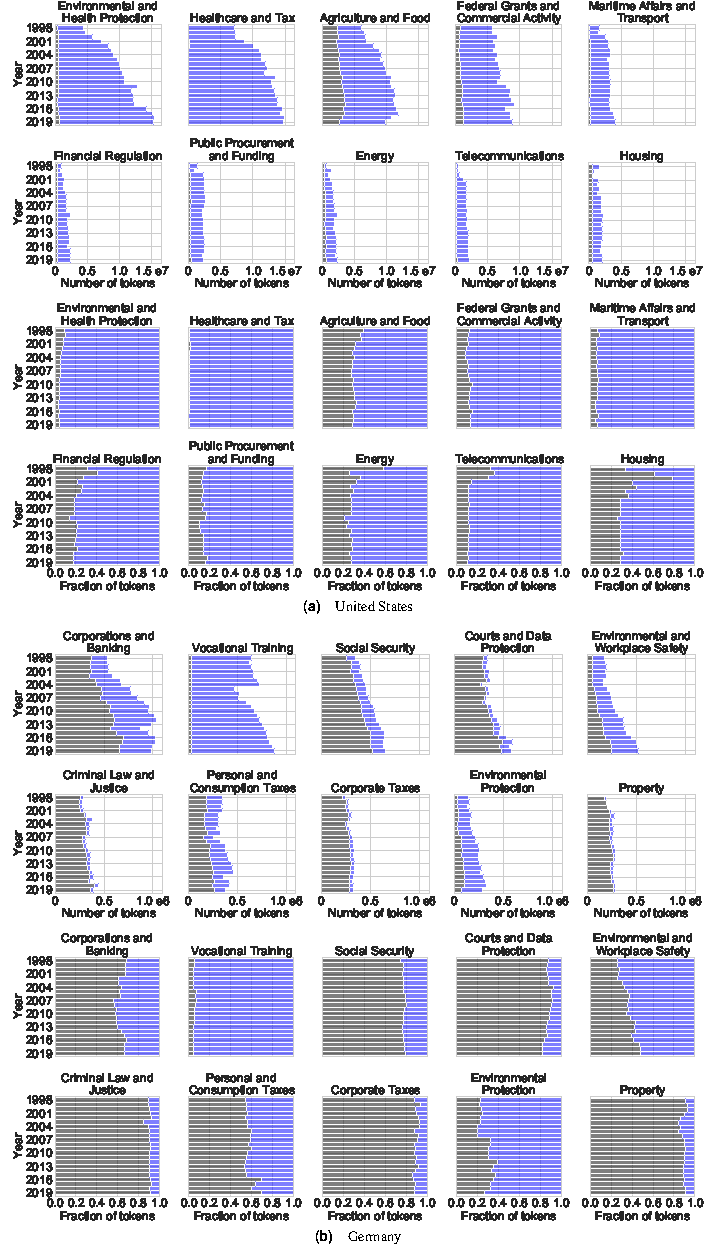
\includegraphics[width=0.75\textwidth]{figure_11}
	\caption{Development of the top ten cluster families from $1998$ to $2019$ as measured by their absolute size in tokens (rows $\{1,2,5,6\}$) and their document type composition (rows $\{3,4,7,8\}$) in the United States (top) and Germany (bottom).
	Black areas represent tokens from statutes and blue areas represent tokens from regulations.}\label{fig:families}
\end{figure}

Inspecting the panels in Figure~\ref{fig:families} in more detail, we observe that the families' ratios of statute tokens to regulation tokens span the whole possible range: 
Some families are \emph{statute-heavy} (i.e., contain mostly statute tokens), 
others are \emph{regulation-heavy} (i.e., contain mostly regulation tokens),
and yet others are \emph{mixed} (i.e., lie between the aforementioned extremes).
For a robust categorization of the ten largest families, the data suggests a threshold of an average $80~\%$ (i.e., an average ratio of $4:1$) over the entire investigation period to classify a family as \emph{x-heavy} for $x\in\{\text{statute}, \text{regulation}\}$.
In the United States, this leads to four mixed families (Agriculture and Food; Financial Regulation; Energy; Housing) and six regulation-heavy families.
In Germany, we find four statute-heavy families (Courts and Data Protection; Criminal Law and Justice; Corporate Taxes; Property), one regulation-heavy family (Vocational Training) and five mixed families.
The overall situation remains similar even if we adopt a simple majority for the classification (eliminating the \emph{mixed} category): 
With the exception of three singular years in two families (Energy in $1998$, and Housing in $1999$ and $2000$), all top families in the United States contain a majority of regulation tokens.
The German data then presents three regulation-heavy families (Vocational Training; Environmental and Workplace Safety; Environmental Protection) and seven statute-heavy families.
A particularly striking example of a statute-heavy family is the Property family in Germany, in which there are nine times as many statute tokens as there are regulation tokens in all years except between $2002$ and $2006$.
The United States cluster family concerning Healthcare and Tax (two topics connected, inter alia, via the tax-based funding of Medicare and Medicaid) represents the opposite extreme, containing almost no statute tokens over the entire period under study.
Interestingly, no family in either country is constantly balanced between statutes and regulations, with the family concerning Personal and Consumption Taxes in Germany coming closest in the period from $1998$ to $2015$.

As Figure~\ref{fig:families} traces the development of the top ten cluster families in each country over time, we can also observe changes in the families' composition.
Extending the terminology adopted above, we can classify the families' growth based on the fraction of growth that is attributable to each of our document types. 
We say that a family is \emph{x-driven} for $x\in \{\text{statute}, \text{regulation}\}$ if tokens from $x$ account for at least $80~\%$ of the family's net growth when comparing $1998$ and $2019$, otherwise, we say that its growth is \emph{mixed}. 
Using these categories, we can classify all of the United States top ten families as regulation-driven
and half of the German top ten families as statute-driven (Social Security; Personal and Consumption Taxes; Criminal Law and Justice; Corporate Taxes; Property), while only one German family is classified as regulation-driven (Vocational Training). 
The full categorization of all top ten families for both countries, both in terms of their average composition and in terms of their growth, can be found in Section~4.3.3 of the~\thesi, 
where we further show that the general tendencies described above also hold for the entire population (although the trends are neither monotone nor universal and their extent differs from family to family).

Overall, the dynamics of the largest cluster families reflect the growth patterns documented in Figure~\ref{fig:basic-statistics}.
In absolute terms, regulations outgrow statutes by large margins in all of the top ten United States families, and statutes moderately outgrow regulations in most of the top ten German families. 
In relative terms, regulations still dominate in the United States, 
and statutes still dominate in Germany (although they are less prominent than they appear when considering absolute numbers).
In summary, based on the top ten families depicted in Figure~\ref{fig:families}, the United States seems to favor rule making via regulations, while Germany seems to favor rule making via statutes, and both countries' preferences appear to get stronger over time.

Finally, to evaluate how federal regulations impact our data-driven map of the United States and German legal systems, we compare the cluster families depicted in Figure~\ref{fig:families} to those derived in prior work that considers only federal statutes \cite{katz2020}.
For the United States, the top ten cluster families based on statutes only have topics similar to those derived from statutes and regulations combined, 
including Environmental and Health Protection, Public Health and Social Welfare, Taxes, Agriculture and Food, Financial Regulation, Public Procurement, Telecommunications, and Federal Grants and Commercial Activity including Small Business Aid.
The topic of Education makes the top ten in the statutes-only data but not in the data containing regulations, while Maritime Affairs and Transport as well as Energy only rise to prominence in the combined data.
In Germany, topics such as Financial Regulation, Taxes, Social Security, Environmental Protection, Criminal Law and Justice, and Property represent sizeable cluster families based on both datasets. 
The topic of Public Servants, Judges, and Soldiers features prominently only in the results excluding regulations, while the families of Vocational Training and of Environmental and Workplace Safety make the top ten only in the combined data.

First and foremost, however, comparing our results to those from \cite{katz2020} demonstrates that adding federal regulations to the data results in a more accurate map of law.
For example, the German data from \cite{katz2020} features a family on Market and Network Regulation that includes a leading cluster on (renewable) energy law, while no comparable family exists in the United States.
Having added federal regulations, we now see such a family in the top ten also in the United States, whose prominent position is explained by its mixed composition (including more than $70~\%$ regulation tokens on average).
At the same time, a cluster concerning (renewable) energy law is now part of the Environmental and Workplace Safety family in Germany because its regulations connect it more closely to rules concerning the protection of the environment than its statutes alone.
This suggests that adding yet further document types, e.g., federal court decisions, to our data will continue to improve the legal maps produced using our methodology, making this a promising avenue for further research.

\vspace*{6pt}
\subsubsection{Micro-level connectivity}
\label{subsubsec:results:connectivity:micro}

We analyze the connectivity of the United States and German legal systems on the micro level in order to identify those code sections that play a particularly important role in mediating the information flow between the sections which they reference and the sections by which they are referenced.
More precisely, we apply the method sketched in Section~\ref{subsec:methods:connectivity} to the graphs induced by the reference edges, where we keep a star if it has at least ten nodes in total. 
We classify these stars (and their hubs) into sinks, hinges, and sources depending on the ratio between their hubs' in-degree and their hubs' out-degree, and hypothesize that hubs of the same type have a similar function within the legal system. 
We explore the merits of this hypothesis by identifying and classifying the stars of each type in $1998$ and $2019$ and analyzing the content of the top five stars (i.e., those with the largest number of nodes) of each type in $2019$ as shown in Table~\ref{tab:structures}.

\begin{table}
	\centering
	% !TeX spellcheck = en_US
\renewcommand{\arraystretch}{1.5}
\renewcommand{\footnotesize}{\fontsize{6.5pt}{8pt}\selectfont}
\footnotesize
	\begin{tabular}{rrrrlp{0.35\textwidth}p{0.35\textwidth}}
\toprule
   $n$ &   $m_S$ &   $\delta^+$ &   $\delta^-$ & \textbf{Type}   & \textbf{Hub}                                                                      & \textbf{Description}   \\
\midrule
  2721 &     933 &            2 &         2719 & Sink            & 5 USC 552 Public information;\newline agency rules, opinions, orders, records, and proceedings                            & Authority to delegate agency rules, records, etc. to regulations                       \\
  \rowcolor{lightgray!30}1702 &      26 &            1 &         1700 & Sink            & 40 CFR 721.125 Recordkeeping requirements                                   & Authority to require particular records to be kept                        \\
  \rowcolor{lightgray!30}1684 &      28 &            3 &         1680 & Sink            & 40 CFR 721.185\newline Limitation or revocation of certain notification requirements& Criteria and procedure for limitation or revocation of notifications by an agency                        \\
  1173 &     298 &            3 &         1171 & Sink            & 5 USC 552a Records maintained on individuals                          & General definitions and procedure for keeping records on individuals                        \\
  \rowcolor{lightgray!30}1023 &      13 &            0 &         1022 & Sink            & 40 CFR 721.80 Industrial, commercial, and consumer activities                & Definition of a new use of a regulated substance                        \\
   283 &      74 &           31 &          254 & Hinge           & 8 USC 1101 Definitions                                          & Definitions for subchapter on immigration and nationality                         \\
   \rowcolor{lightgray!30}218 &     150 &          114 &          213 & Hinge           & 49 CFR 171.7 Reference Material                                              & Collection of materials to be incorporated by reference in other subchapters                       \\
   \rowcolor{lightgray!30}141 &      34 &           34 &          127 & Hinge           & 49 CFR 172.101 Purpose and use of hazardous materials table                  & Collection of substances deemed hazardous materials                       \\
   138 &      18 &           20 &          117 & Hinge           & 10 USC 101 Definitions                                                   & Definitions including bundling of statutes                       \\
   127 &       8 &           24 &          103 & Hinge           & 15 USC 637 Additional Powers                                              & Authority to carry out actions required throughout the chapter                      \\
   \rowcolor{lightgray!30}215 &      23 &          213 &            1 & Source          & 7 CFR 2.22\newline Under Secretary for Marketing and Regulatory Programs            & Enumeration of stand-in duties contained in other statutes                       \\
   \rowcolor{lightgray!30}177 &      13 &          174 &            2 & Source          & 7 CFR 2.21\newline Under Secretary for Research, Education, and Economics            &  Enumeration of stand-in duties contained in other statutes                      \\
   \rowcolor{lightgray!30}150 &      36 &          149 &            0 & Source          & 19 CFR 178.2 Listing of OMB control numbers                                 & Mapping of documents in other parts to control numbers from the Office of Management and Budget                      \\
   \rowcolor{lightgray!30}133 &      16 &          128 &            4 & Source          & 7 CFR 2.16 Under Secretary for Farm Production and Conservation              & Enumeration of stand-in duties contained in other statutes                     \\
   \rowcolor{lightgray!30}129 &       8 &          128 &            0 & Source          & 7 CFR 2.79 Administrator, Agricultural Marketing Service                     & Enumeration of stand-in duties contained in other statutes                          \\
\bottomrule
\end{tabular}
			
{\vspace*{3pt}\small \textbf{\textsf{(a)}}\quad United States}\vspace*{6pt}
	
\begin{tabular}{rrrrlp{0.35\textwidth}p{0.35\textwidth}}
\toprule
   $n$ &   $m_S$ &   $\delta^+$ &   $\delta^-$ & \textbf{Type}   & \textbf{Hub}                                                                            & \textbf{Description}   \\
\midrule
   256 &      19 &            0 &          255 & Sink            & § 36 Gesetz über Ordnungswidrigkeiten                                                   & Determination of the competent authority to prosecute misdemeanor   \\
   224 &       6 &            0 &          223 & Sink            & § 4 Berufsbildungsgesetz                                                                & Authority to delegate vocational training regulations (professions)                      \\
   194 &       0 &            1 &          192 & Sink            & § 25 Gesetz zur Ordnung des Handwerks                                                   & Authority to delegate vocational training regulations (crafts)                        \\
   191 &       3 &            0 &          190 & Sink            & § 1 Berufsbildungsgesetz                                                                & Goal and definitions for vocational training                      \\
   180 &      24 &           16 &          168 & Sink            & § 1 Gesetz über das Kreditwesen                                                         & Definitions for financial and banking regulation                       \\
   131 &      27 &           88 &           46 & Hinge           & § 3 Einkommensteuergesetz                                                               & Enumeration of tax-free income types                       \\
    88 &       0 &           74 &           13 & Hinge           & Art 229 Weitere Überleitungsvorschriften\newline Einführungsgesetz zum Bürgerlichen Gesetzbuche & Transitional provisions of the civil code                       \\
    86 &       1 &           18 &           68 & Hinge           & § 60 Lebensmittel-, Bedarfsgegenstände-\newline und Futtermittelgesetzbuch                      & Misdemeanors in food and feed safety                       \\
    84 &       0 &           73 &           10 & Hinge           & Art 97 Übergangsvorschriften\newline Einführungsgesetz zur Abgabenordnung                       & Transitional provisions of the fiscal code                       \\
    82 &       0 &           61 &           20 & Hinge           & § 100a Strafprozeßordnung                                                               & Definition of particularly serious crimes\newline allowing for telecommunication surveillance                       \\
    \rowcolor{lightgray!30}76 &       0 &           75 &            0 & Source          & § 69a Straßenverkehrs-Zulassungs-Ordnung                                                & Misdemeanors in traffic and road safety                       \\
    73 &       1 &           71 &            2 & Source          & § 340 Kapitalanlagegesetzbuch                                                           & Misdemeanors in the capital investment code                        \\
    59 &       0 &           56 &            2 & Source          & § 194 Gesetz zum Schutz vor der schädlichen Wirkung\newline ionisierender Strahlung             & Misdemeanors in the radiation protection statute                      \\
    \rowcolor{lightgray!30}48 &       0 &           47 &            0 & Source          & § 184 Verordnung zum Schutz vor der schädlichen Wirkung\newline ionisierender Strahlung         & Misdemeanors in the radiation protection regulation                       \\
    48 &       1 &           45 &            3 & Source          & § 120 Gesetz über den Wertpapierhandel                                                  & Misdemeanors and authority to delegate in the securities trading act                       \\
\bottomrule
\end{tabular}



				
{\vspace*{3pt}\small \textbf{\textsf{(b)}}\quad Germany}

	\caption{%
		Top five reference stars of each type in $2019$ for the United States (top) and Germany (bottom), 
		with stars whose hubs are contained in regulations marked grey.
		Edge and degree counts exclude multi-edges; 
		$m_S$ is the number of edges between spokes, 
		$\delta^+$ is the hub's out-degree, 
		and $\delta^-$ is the hub's in-degree.
	}\label{tab:structures}
	\vspace*{-6pt}
\end{table}

In the United States, we find that hubs of the same type indeed play similar roles in the legal system: 
\emph{Sinks} contain delegation of authority and general procedures, e.g., for record keeping, that are relevant for and therefore referenced by many other sections.
\emph{Hinges} connect entire collections, enumerations, and definitions to one another. 
49~CFR~§~171.7 is an example, as its only function is the incorporation of material collections by external parties (such as the American National Standards Institute) into other sections of the CFR like 49~CFR~§~173.306, which itself serves as a hub for other sections. 
\emph{Sources} enumerate duties contained in other statutes (four of the top five stem from the CFR title on Agriculture, in which this drafting technique seems to be popular) or provide a document map for their respective chapter. 

In Germany, the results paint a similar picture:
\emph{Sinks} contain provisions for delegation of legislative authority (as expected by legal theory), competencies, statements of goals, or definitions.
\emph{Hinges} contain transitional provisions, 
which are designed to bridge between old and new rules, as well as definitions.
The definition classified as a hinge (§~100a Strafprozeßordnung) establishes a well-known connection between the Criminal Code and its definition of crimes and investigative methods described both inside and outside the Code of Criminal Procedure.
All \emph{sources} (and one hinge) are collections of misdemeanors to sanction violations of rules contained in their respective statute or regulation, 
and they encompass activities as diverse as road traffic, securities trading, and handling radioactive materials.
Hence, our classification correctly identifies examples of this popular drafting technique.

As suggested in Section~\ref{subsubsec:methods:connectivity:micro} and confirmed for the largest stars, the type of a star contains information about a section's function within the legal system.
Examining the hundred largest stars, whose types are shown in Table~\ref{tab:star-statistics}, exposes different trends in both countries.
In the United States, sinks dominate both across document types and over time, accounting for three out of four stars in $1998$ and six out of seven stars in $2019$, which points to a pronounced drafting preference.
At the local level, sections of the United States codified law are mostly connected (only) by referencing the same section, which often contains a definition or the description of a procedure.
In Germany, the composition is more balanced to begin with, but sinks still make up the largest share in $1998$. 
Over time, though, the number of sinks and sources amongst the hundred largest stars decreases in favor of hinges. 
Hence, individual sections are no longer only connected by a reference to the same section, but the frequently referenced sections themselves increasingly reference other sections.
As a consequence, the number of sections that are reachable from any individual section in two hops (i.e., following two references) increases.
This makes the information flow via references more efficient, which could explain the reduced need for structural elements to guide information flow via hierarchy in Germany when compared to the United States.
But it also increases the prevalence of reference chains, possibly making the German legal system progressively harder to navigate.

\begin{table}
	\centering
	% !TeX spellcheck = en_US
\renewcommand{\arraystretch}{1.5}
\begin{multicols}{2}
	\begin{tabular}{rrrrr}
\toprule&\multicolumn{2}{c}{\textbf{1998}}&\multicolumn{2}{c}{\textbf{2019}}\\
        &   \textbf{S-Hub} &   \textbf{R-Hub} &   \textbf{S-Hub} &   \textbf{R-Hub} \\
\midrule
   \textbf{Sink} &           60 &           16 &           56 &           30 \\
  \textbf{Hinge} &            8 &            1 &            6 &            3 \\
 \textbf{Source} &            0 &           15 &            0 &            5 \\
\bottomrule
\end{tabular}

	{\vspace*{6pt}\small \textbf{\textsf{(a)}}\quad United States}\vspace*{6pt}
	\newpage
	\begin{tabular}{rrrrr}
\toprule&\multicolumn{2}{c}{\textbf{1998}}&\multicolumn{2}{c}{\textbf{2019}}\\
        &   \textbf{S-Hub} &   \textbf{R-Hub} &   \textbf{S-Hub} &   \textbf{R-Hub} \\
\midrule
   \textbf{Sink} &           42 &            0 &           33 &            0 \\
  \textbf{Hinge} &           30 &            0 &           52 &            1 \\
 \textbf{Source} &           17 &           11 &            8 &            6 \\
\bottomrule
\end{tabular}
	
	{\vspace*{6pt}\small \textbf{\textsf{(b)}}\quad Germany}
\end{multicols}

	\caption{%
		Types of the top hundred reference stars (i.e., those with the largest number of nodes) in $1998$ and $2019$ for the United States (left) and Germany (right). S-Hubs are hubs contained in statutes and R-Hubs are hubs contained in regulations.
	}\label{tab:star-statistics}
\end{table}

Mirroring the larger trends described in Section~\ref{subsubsec:results:connectivity:macro} and Section~\ref{subsubsec:results:connectivity:meso}, regulations play a more important role in the United States than in Germany at the micro level of connectivity as well. 
While the total share of regulation hubs in Germany is small, 
they make up almost half of the sources amongst the top hundred reference stars in $2019$, which again follows the larger pattern of regulations referencing rather than being referenced.
In the United States, regulation hubs account for just under $40~\%$ of the top hundred reference stars, 
but almost all of the largest stars are sinks, regardless of the document type of their hub.
This suggests that the United States drafting dynamics resulting in sinks affect both the executive and the legislative branches of government. 

\vspace*{6pt}
\subsection{Profiles}
\label{subsec:results:profiles}

In a step toward developing a dashboard for measuring and monitoring the law, 
we demonstrate the utility of the profiling procedure described in Section~\ref{subsec:methods:profiles} by applying it to selected statutes and regulations from the United States and Germany in a case study focusing on financial regulation. 
We profile a total of four statutes (two from each country) that constitute landmark legislation in this domain and trace their statistics over time in Figure~\ref{fig:profiles}, 
along with those of two additional regulations from the same area.

\begin{figure}
	\centering
	\vspace*{-8pt}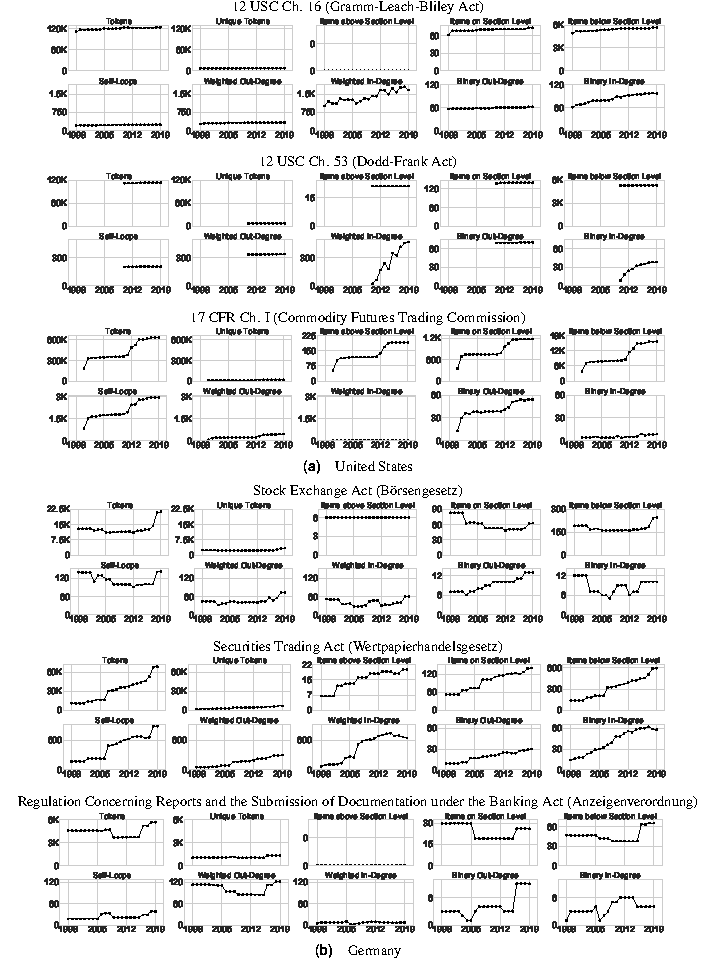
\includegraphics[width=\textwidth]{figure_12}\vspace{-6pt}
	\caption{%
		Profiles tracking the evolution of selected laws related to financial regulation for the United States (top) and Germany (bottom) from $1998$ to $2019$.
	}\label{fig:profiles}
\end{figure}

12~USC~Ch.~16, popularly known as the Gramm-Leach-Bliley Act or Financial Services Modernization Act of 1999 (GLBA), liberalized the United States financial market by allowing the combination of investment banks, commercial banks, and insurance companies in one institution. 
It has been in effect for nearly our entire investigation period ($1999$--$2019$) and, as indicated by nearly flat lines in all but the panels related to in-degree, has not materially changed.
However, the interaction of the GLBA with other parts of the legal system has been anything but static, with its initial weighted in-degree of $1000$ increasing by $60~\%$ between $1999$ and $2019$ due to incoming references from other statutes and regulations.
Unlike the growth trend in the weighted in-degree, the growth trend in the binary in-degree is nearly monotonic. 
This indicates that most of the fluctuations in the GLBA's regulatory environment occur within individual chapters of the USC or the CFR.
In summary, the GLBA can therefore be rightfully regarded as a landmark statute, which has required little engineering but has remained an important reference throughout the period under study.

The profile of 12~USC~Ch.~53, popularly known as the Dodd-Frank Act or the Wall Street Reform and Consumer Protection Act (DFA), shows similarities with the GLBA in most statistics we track.
Introduced in response to the Great Recession in $2010$, 
it is approximately half as old as the GLBA, 
and like the GLBA, it has barely changed in size, breadth, or structure.
But although the DFA is comparable to the GLBA in size, 
its interaction with the environment seems much more dynamic, 
with its weighted in-degree increasing by a factor of almost ten over its lifetime.
In absolute terms, however, the references increase by less than $500$, i.e., in the same order of magnitude as for the GLBA.
This is in line with the fact that both statutes are part of the same legal domain, and it highlights how much the evolution of individual pieces of legislation is influenced by their initial conditions, e.g., whether they are strongly connected with their environment already at birth.
For the DFA, the growth of the weighted in-degree again is not monotonic, 
but it is visibly steeper before $2017$ than afterwards, leveling off in the last years of the period under study.
The binary in-degree, whose gradient is almost monotonically decreasing from the start, anticipates this deceleration by several years.
This suggests the existence of an onboarding period, in which the DFA is integrated into the regulatory environment before finding its place in the United States legal system (see the related discussion in \cite{mclaughlin2021}).

The profiles of the two German statutes we examine are starkly different from those of the United States statutes.
Statutes under the names of both the Stock Exchange Act (SEA) and the Securities Trading Act (STA) have been in effect for the entire observation period.
As indicated by their unique token count, they are both constantly narrow in thematic scope (with the STA an order of magnitude more narrow than the SEA to start with), 
and their token count increases over time.
While the SEA and the STA start at comparable sizes in $1998$, the STA grows by a factor of seven, while the SEA merely doubles.
Possibly as a result, the SEA largely maintains its original number of structures,
while the number of structural elements in the STA triples.
This is accompanied by an expected, nearly parallel increase in the number of STA sections, 
and even a decrease of about $25~\%$ in the number of SEA sections.
Beyond the general growth trends present in almost all STA statistics,
the period from $2006$ to $2007$ stands out, as most of its statistics experience a relatively steep increase between these years.
The doctrinal investigation prompted by this observation reveals that the source of the increases is a legislative project translating extensive transparency requirements mandated by the European Union into German law (Transparenzrichtlinie-Umsetzungsgesetz), which came into effect in January $2007$.
This finding also shows how our methods can complement doctrinal legal scholarship, as has been demonstrated, e.g., for the development of the STA over its entire lifetime \cite{coupette2019a}.

Our statistics produce interesting insights not only for statutes but also for regulations.
For example, there is a noticeable increase in the self-referentiality of the CFR chapter about the Commodity Futures Trading Commission (CFTCR),
and the German Reports and Documents Regulation (RDR) shows structural changes between $2005$ and $2006$ as well as between $2015$ and $2016$.
As our framework enables the joint modeling of data from different document types, its application can surface characteristic differences between these types, too.
Examining our exemplary regulations and statutes in Figure~\ref{fig:profiles},
we find that the CFTCR experiences noticeable growth (about $200~\%$),
while the size of the featured statutes barely changes.
At the same time, the regulation's weighted in-degree is several orders of magnitude smaller than that of the DFA or the GLBA, supporting the intuition that statutes should be referenced more frequently than regulations for this particular case. 
In Germany, the RDR is smaller than the featured German statutes,
and it covers less diverse content (as would be expected for a regulation from a legal theory perspective).
Its structural organization is minimal, as is its self-referentiality.
This confirms that smaller units of law require less internal organization by both structure and references.
The RDR references, and is referenced by, a small number of different documents, indicating homogeneity in its regulatory environment.
Its weighted out-degree falls between the SEA and STA, i.e., it has a non-negligible number of references to a limited number of targets.
In summary, the RDR has most characteristics expected from a German regulation, and its overall profile can clearly be distinguished from that of the featured German statutes.

Our framework enables comparisons not only across document types but also across countries.
When examining the DFA and the STA, we see that the STA starts at a size of roughly a third of the DFA but grows to two thirds of the DFA over time.
Both statutes have similar degrees of structure at the section level and above,
but the DFA contains ten to fifteen times the amount of items below section level, indicating a vastly more granular hierarchical organization.
Conversely, the STA contains three to four times more self-loops than the DFA, with its weighted in-degree about $1.5$ times and its binary in-degree between $1.5$ and $2$ times higher than those of the DFA after the first couple of years.
This mirrors the more general finding that rule-making agents in the United States and Germany favor different mechanisms to handle the token growth of their statutory corpora: 
Americans like adding hierarchical structure, while Germans prefer adding references \cite{katz2020}.

Figure~\ref{fig:profile-graphs} combines profile statistics concerning size and interdependence to enable direct visual comparisons. 
Here, we compare the ego graphs of the DFA and the STA for every quarter of their existence during our investigation period.
Note that the distance between the snapshots is different for both statutes, 
as the DFA was adopted only in the middle of our study period, but both series end in $2019$.
Complementing the statistics presented in Figure~\ref{fig:profiles}, the visualization attributes the references to their actual sources and targets, indicating their number by the weight of the edges.
For the DFA, its \emph{reliance} (i.e., how much and how diversely it references other statutes and regulations) barely changes,
while its \emph{responsibility} (i.e., how much and how diversely it is referenced by other statutes and regulations) discernibly increases, 
as the DFA becomes more and more integrated with its environment.
In contrast, both the reliance and the responsibility of the STA increase over time, with its responsibility starting nearly twice as high and increasing at a much faster rate than its reliance.
As shown by the edge colors, the diverse responsibility of the STA concerns both statutes and regulations,
and the DFA is most intensively responsible for regulations.
In line with the expectation derived from legal theory,
both the DFA and the STA rely mostly on statutes.

\begin{figure} 
	\centering
	\vspace*{-8pt}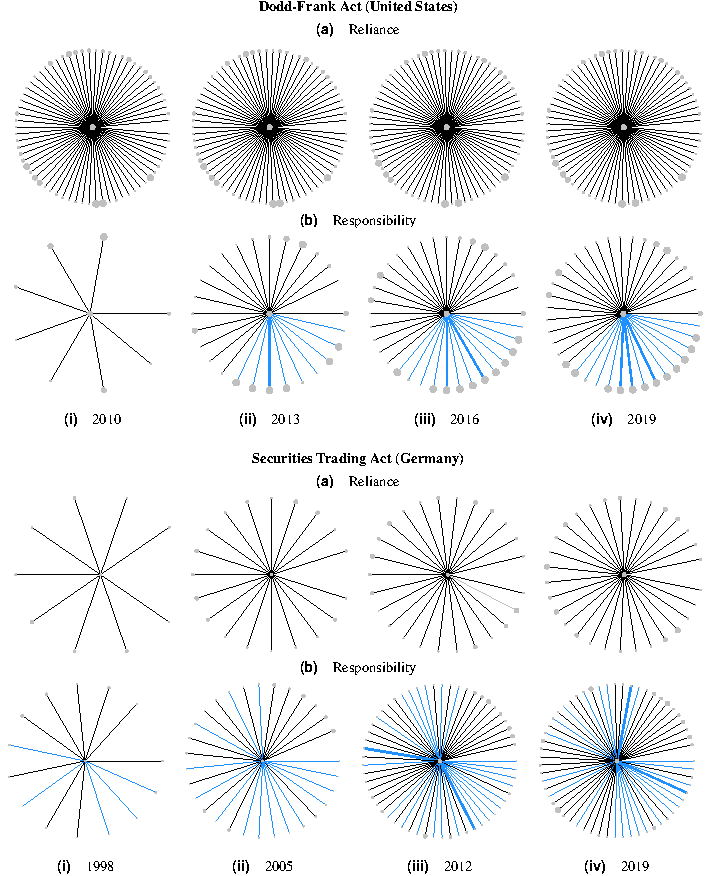
\includegraphics[width=\textwidth]{figure_13}
	\caption{Reliance and responsibility of the Dodd-Frank Act (DFA, top) and the Securities Trading Act (STA, Wertpapierhandelsgesetz, bottom) from $1998$ to $2019$.
	Leaf nodes are chapters of the USC or the CFR that are cited by (reliance) or cite (responsibility) the DFA (top), 
	and statutes or regulations (or their books, if applicable) that are cited by (reliance) or cite (responsibility) the STA (bottom).
	Edge types indicate reference types as used in Figure~\ref{fig:crossref-differentiation} (black for lateral statute references, light blue for upward references, and silver for downward references).
	Node size is proportional to the node's number of tokens;
	edge width is proportional to the number of references represented by the edge.
	}\label{fig:profile-graphs}
\end{figure}


% !TeX spellcheck = en_US
% !TeX root = ../main.tex
\section{Discussion}
\label{sec:discussion}

We have introduced an analytical framework for the dynamic network analysis of legal documents and demonstrated its utility by applying it to a dataset comprising federal statutes and regulations in the United States and Germany over a period of more than $20$ years.
The limitations of this work concern two separate areas: 
the methods introduced in Section~\ref{sec:methods} and the results presented in Section~\ref{sec:results}.

To gravitate toward its ideal formulation, our framework requires further refinement based on experiences from applications to diverse datasets.
Our model is deliberately document type and country agnostic, such that it can be easily instantiated for new data. 
Similar studies using legal documents from a variety of jurisdictions would be of immense value for improving our framework, 
and they could provide further context for the results reported in Section~\ref{sec:results}.
Furthermore, our network analytical framework could be complemented by a framework for natural legal language processing, 
as the combination of relational information and linguistic information will likely lead to insights that would not be possible using either of these sources alone.

When preparing this article, we found that combining documents of different types in one graph representation raises many conceptual questions.
Some of these questions relate to the presentation of our results, e.g., 
whether to depict dynamics in absolute or relative terms (thereby either impairing comparisons across document types of different sizes or visually overstating dynamics for small baselines).
Others concern design decisions when defining our methods, 
e.g., whether tokens from documents of different types should have the same weight when determining cluster families even if there is a striking imbalance between the total number of tokens in documents of these types (as is the case in our United States data).
Here, one alternative would be to rescale the token counts before constructing the cluster family graph, 
such that the total influence of tokens from one specific document type is equal across all types.
While this would change the results to a certain extent, 
it is difficult to assess whether the modified method would be superior because comparable investigations of multimodal legal document networks currently do not exist.

The results stated in Section~\ref{sec:results} are limited in geographic scope (United States and Germany), temporal scope ($1998$--$2019$), and institutional scope (legislative and executive branch on the federal level).
Most importantly, our findings cover only codified law.
As the United States and Germany are typically assumed to follow distinct legal traditions (common law and civil law), 
which are often thought to differ, inter alia, in their reliance on court precedent, including court decisions might have disparate impact on our results for both countries.
However, it could also provide empirical evidence against the traditional classification.
Irrespective of legal traditions, unlocking and integrating judicial data is an important direction for future work.

Regarding both growth and connectivity, the next steps consist in eliminating the uncertainties and limitations affecting our data.
For example, as highlighted in Section~\ref{subsec:data:instance}, one important stride toward a more comprehensive picture of the connectivity between legal documents is the extraction and resolution of non-atomic references.
At the macro level, connectivity could also be evaluated at other resolutions (e.g., the chapter level) or when including hierarchy edges, 
and our analysis could be expanded using further statistics, such as motif counts and their evolution over time.
Furthermore, applying our methods to other document types or other countries would help us assess whether the rocket structure we found in our data is characteristic of legal systems in general.
When assessing connectivity at the meso level, the dynamic map of law provided by our cluster families could be further refined, especially at other resolution levels.
At the micro level of connectivity, a more fine-grained star taxonomy might be in order because in both countries, there exists some functional overlap between hinge stars and sink stars.
For the profiles, a sensible step forward would be to apply the tracing methodology at other levels of resolution (e.g., at the level of individual sections), and the statistics we track could be complemented by similarity measures allowing us to compare between the different units of law we analyze.

Beyond the specific opportunities for further research outlined above, 
our work raises three larger questions to be explored in the future:
\begin{enumerate}
	\item \emph{When quantitatively analyzing legal documents, how should we choose the unit of analysis?}\\
	On the one hand, no clear consensus exists as to what constitutes a \emph{unit of law} or a \emph{legal rule}. 
	But on the other hand, the choice has far-reaching consequences for all analyses.
	Furthermore, even analyzing all documents at the same structural level presents problems: 
	Legal rules come in various sizes, and at times, a single paragraph might be longer than the average document due to drafting decisions by the agents in the legal system.
	This complicates comparisons and creates countless opportunities for erroneous interpretations.
	Detailing the full rationale behind all choices we made when presenting our results in Section~\ref{sec:results} is beyond the scope of this article. 
	However, an extensive exposition of the possible choices and the tradeoffs surrounding them would benefit the research community at large and, therefore, constitutes a fecund field for future findings.
	\item \emph{How can we measure the \emph{regulatory energy} of statutes?}\\
	The analysis of individual statutes such as the Gramm-Leach-Bliley Act and the Dodd-Frank Act suggests that legislative outputs impact their environments at potentially different rates (e.g., by prompting further rule making), 
	i.e., that they have a certain \emph{regulatory energy} that they emit over time. 
	This hypothesis could be validated, inter alia, using external data on regulatory relevance, e.g., the filings concerning regulatory risk that are required for annual and transition reports pursuant to sections 13 or 15(d) of the Securities Exchange Act of $1934$ under 17~CFR~249.310 -- Form 10-K \cite{bommarito2017}. 
	However, other approaches are equally possible and merit further investigation.
	\item \emph{How can we connect our empirical findings to established theories in law and political science?}\\
	Although beyond the scope of this work, some of our findings can be combined with analyses using established theories on the composition and evolution of codified law in both legal scholarship and political science.
	The most prominent example here is the question of delegation: 
	How does it happen and what are its limits, in theory and in practice?
	This touches the heart of democratic legitimacy, and it presents a promising opportunity for empirical legal studies to contribute to mainstream legal and political science discourse that we are planning to seize in the future.
\end{enumerate}



%For Original Research Articles \citep{conference}, Clinical Trial Articles \citep{article}, and Technology Reports \citep{patent}, the introduction should be succinct, with no subheadings \citep{book}. For Case Reports the Introduction should include symptoms at presentation \citep{chapter}, physical exams and lab results \citep{dataset}.



%\section{Article types}
%
%For requirements for a specific article type please refer to the Article Types on any Frontiers journal page. Please also refer to  \href{http://home.frontiersin.org/about/author-guidelines#Sections}{Author Guidelines} for further information on how to organize your manuscript in the required sections or their equivalents for your field
%
%% For Original Research articles, please note that the Material and Methods section can be placed in any of the following ways: before Results, before Discussion or after Discussion.

%\section{Manuscript Formatting}
%
%\subsection{Heading Levels}
%
%%There are 5 heading levels
%
%\subsection{Level 2}
%\subsubsection{Level 3}
%\paragraph{Level 4}
%\subparagraph{Level 5}
%
%\subsection{Equations}
%Equations should be inserted in editable format from the equation editor.
%
%\begin{equation}
%\sum x+ y =Z\label{eq:01}
%\end{equation}
%
%\subsection{Figures}
%Frontiers requires figures to be submitted individually, in the same order as they are referred to in the manuscript. Figures will then be automatically embedded at the bottom of the submitted manuscript. Kindly ensure that each table and figure is mentioned in the text and in numerical order. Figures must be of sufficient resolution for publication \href{http://home.frontiersin.org/about/author-guidelines#ResolutionRequirements}{see here for examples and minimum requirements}. Figures which are not according to the guidelines will cause substantial delay during the production process. Please see \href{http://home.frontiersin.org/about/author-guidelines#GeneralStyleGuidelinesforFigures}{here} for full figure guidelines. Cite figures with subfigures as figure \ref{fig:2}B.


%\subsubsection{Permission to Reuse and Copyright}
%Figures, tables, and images will be published under a Creative Commons CC-BY licence and permission must be obtained for use of copyrighted material from other sources (including re-published/adapted/modified/partial figures and images from the internet). It is the responsibility of the authors to acquire the licenses, to follow any citation instructions requested by third-party rights holders, and cover any supplementary charges.
%%Figures, tables, and images will be published under a Creative Commons CC-BY licence and permission must be obtained for use of copyrighted material from other sources (including re-published/adapted/modified/partial figures and images from the internet). It is the responsibility of the authors to acquire the licenses, to follow any citation instructions requested by third-party rights holders, and cover any supplementary charges.

%\subsection{Tables}

%Tables should be inserted at the end of the manuscript. Please build your table directly in LaTeX.Tables provided as jpeg/tiff files will not be accepted. Please note that very large tables (covering several pages) cannot be included in the final PDF for reasons of space. These tables will be published as \href{http://home.frontiersin.org/about/author-guidelines#SupplementaryMaterial}{Supplementary Material} on the online article page at the time of acceptance. The author will be notified during the typesetting of the final article if this is the case. 

%\section{Nomenclature}
%
%\subsection{Resource Identification Initiative}
%To take part in the Resource Identification Initiative, please use the corresponding catalog number and RRID in your current manuscript. For more information about the project and for steps on how to search for an RRID, please click \href{http://www.frontiersin.org/files/pdf/letter_to_author.pdf}{here}.
%
%\subsection{Life Science Identifiers}
%Life Science Identifiers (LSIDs) for ZOOBANK registered names or nomenclatural acts should be listed in the manuscript before the keywords. For more information on LSIDs please see \href{http://www.frontiersin.org/about/AuthorGuidelines#InclusionofZoologicalNomenclature}{Inclusion of Zoological Nomenclature} section of the guidelines.


%\section{Additional Requirements}
%
%For additional requirements for specific article types and further information please refer to \href{http://www.frontiersin.org/about/AuthorGuidelines#AdditionalRequirements}{Author Guidelines}.

\section*{Conflict of Interest Statement}

DMK and MB are affiliated with the start-up LexPredict, which is now part of Elevate Services.
CC, JB, and DH declare that the research was conducted in the absence of any commercial or financial relationships that could be construed as a potential conflict of interest.

\section*{Author Contributions}

All authors conceived of the research project. CC, JB, and MB performed the computational analysis in consultation with DMK and DH.
CC, DH, and MB drafted the manuscript, which was revised and reviewed by all authors. All authors gave final approval for publication and agree to be held accountable for the work performed therein.

% The Author Contributions section is mandatory for all articles, including articles by sole authors. If an appropriate statement is not provided on submission, a standard one will be inserted during the production process. The Author Contributions statement must describe the contributions of individual authors referred to by their initials and, in doing so, all authors agree to be accountable for the content of the work. Please see  \href{http://home.frontiersin.org/about/author-guidelines#AuthorandContributors}{here} for full authorship criteria.

% \section*{Funding}
% Details of all funding sources should be provided, including grant numbers if applicable. Please ensure to add all necessary funding information, as after publication this is no longer possible.

% \section*{Acknowledgments}
% This is a short text to acknowledge the contributions of specific colleagues, participation, or agencies that aided the efforts of the authors.

\section*{Supplemental Data}

The supplemental material for this paper is archived under the following DOI:\\ 
\tbd

\section*{Data Availability Statement}

For the United States, the raw input data used in this study is publicly available from the Annual Historical Archives published by the Office of the Law Revision Counsel of the U.S. House of Representatives and the United States Government Publishing Office, and is also available from the authors upon reasonable request. 
For Germany, the raw input data used in this study was obtained from \emph{juris GmbH} but restrictions apply to the availability of this data, which was used under license for the current study, and so is not publicly available. 
For details, see Section~1 of the \thesi. 
The preprocessed data used in this study (for both the United States and Germany) is archived under the following DOI:\\ \url{https://doi.org/10.5281/zenodo.4660133}

\section*{Code Availability Statement}

The code used in this study is available on GitHub in the following repositories: 
\begin{itemize}
	\item Paper: \url{https://github.com/QuantLaw/Measuring-Law-Over-Time}\\
	DOI of publication release: \url{https://doi.org/10.5281/zenodo.4660191}
	\item Data preprocessing: \url{https://github.com/QuantLaw/legal-data-preprocessing}\\
	DOI of publication release: \url{https://doi.org/10.5281/zenodo.4660168}
	\item Clustering: \url{https://github.com/QuantLaw/legal-data-clustering}\\
	DOI of publication release: \url{https://doi.org/10.5281/zenodo.4660184}
\end{itemize}

% Please see the availability of data guidelines for more information, at https://www.frontiersin.org/about/author-guidelines#AvailabilityofData

%\bibliographystyle{frontiersinSCNS_ENG_HUMS} % for Science, Engineering and Humanities and Social Sciences articles, for Humanities and Social Sciences articles please include page numbers in the in-text citations
\bibliographystyle{frontiersinHLTH&FPHY} % for Health, Physics and Mathematics articles
\bibliography{bibliography}

%%% Make sure to upload the bib file along with the tex file and PDF
%%% Please see the test.bib file for some examples of references

%\section*{Figure captions}

%%% Please be aware that for original research articles we only permit a combined number of 15 figures and tables, one figure with multiple subfigures will count as only one figure.
%%% Use this if adding the figures directly in the mansucript, if so, please remember to also upload the files when submitting your article
%%% There is no need for adding the file termination, as long as you indicate where the file is saved. In the examples below the files (logo1.eps and logos.eps) are in the Frontiers LaTeX folder
%%% If using *.tif files convert them to .jpg or .png
%%%  NB logo1.eps is required in the path in order to correctly compile front page header %%%

%\begin{figure}[h!]
%\begin{center}
%%
\includegraphics[width=10cm]{logo1}% This is a *.eps file
%\end{center}
%\caption{ Enter the caption for your figure here.  Repeat as  necessary for each of your figures}\label{fig:1}
%\end{figure}


%\begin{figure}[h!]
%\begin{center}
%%\includegraphics[width=15cm]{logos}
%\end{center}
%\caption{This is a figure with sub figures, \textbf{(A)} is one logo, \textbf{(B)} is a different logo.}\label{fig:2}
%\end{figure}

%%% If you are submitting a figure with subfigures please combine these into one image file with part labels integrated.
%%% If you don't add the figures in the LaTeX files, please upload them when submitting the article.
%%% Frontiers will add the figures at the end of the provisional pdf automatically
%%% The use of LaTeX coding to draw Diagrams/Figures/Structures should be avoided. They should be external callouts including graphics.

\end{document}
